\documentclass[DM,lsstdraft,authoryear,toc]{lsstdoc}
% lsstdoc documentation: https://lsst-texmf.lsst.io/lsstdoc.html

% Package imports go here.
\usepackage{booktabs}
\usepackage{xspace}
\usepackage{hyperref}
\usepackage{graphicx}

% Local commands go here.
\newcommand{\opsim}{\texttt{OpSim}\xspace}
\newcommand{\socs}{\texttt{SOCS}\xspace}
\newcommand{\sched}{\texttt{Scheduler}\xspace}
\newcommand{\simsky}{\texttt{sims\_skybrightness}\xspace}
\newcommand{\magasq}{magnitude/arcsecond$^{2}$\xspace}

% To add a short-form title:
% \title[Short title]{Title}
\title{A New Baseline Operations Simulation}

% Optional subtitle
% \setDocSubtitle{A subtitle}

\author{%
Lynne Jones,
Owen Boberg,
Tiago Ribeiro, \\
Kem Cook,
Francisco Delgado,
Andrew Heyer, \\
\v{Z}eljko Ivezi\'{c},
Michael Reuter,
Colin Winslow
}

\setDocRef{baseline-opsim}

\date{\today}

% Optional: name of the document's curator
% \setDocCurator{The Curator of this Document}

\setDocAbstract{%
We present an update to the baseline simulated survey, created using \opsim v4.1.0.10. The last \opsim baseline simulated survey was minion\_1016, produced in 2016 using \opsim v3.3.5 The changes in the new baseline run include updates to the sky brightness, significant changes in the underlying opsim scheduling software, and the addition of new scheduler parameters.
}

% Change history defined here.
% Order: oldest first.
% Fields: VERSION, DATE, DESCRIPTION, OWNER NAME.
% See LPM-51 for version number policy.
\setDocChangeRecord{%
  \addtohist{1}{YYY-MM-DD}{Unreleased.}{Lynne Jones}
}

\begin{document}

% Create the title page.
% Table of contents is added automatically with the "toc" class option.
\maketitle

\section{Overview}

The new \opsim v4 codebase makes significant changes when compared with the previous \opsim v3 software. These include:
\begin{itemize}
\item Separation of the telemetry and telescope control simulation software from the scheduler software. These two packages are now called \texttt{Simulated Observatory Control System} (\socs) and \texttt{Scheduler}.
\item Implement communication between \socs and \sched via DDS, a publish/subscribe protocol that will be used to communicate between various telescope control systems, including the scheduler code.
\item Add a per-filter sky brightness calculation, using the \simsky package to calculate sky brightness values. This updates the sky brightness values to a model that includes a much higher fidelity twilight component and which has been validated against all-sky measurements from the LSST site. It also means that for each visit, the sky brightness limit is compared against the actual sky brightness estimate in the individual filter, instead of just against the $V$ band sky brightness as in \opsim v3.
\item Update the slew time cost function, to add further flexibility to prioritize short slews.
\item Add an additional cost to changing the filter, to reduce the number of filter changes and in particular, fast filter changes.
%\item Add the capability to restrict observations to a specified number of visits in a particular filter for a given field, per night. {\it E.g.}, limit visits for a given field to only 2 in $g$ band. This does not mean that no other visits to the same field will take place in the same night, but they would be in other filters which still have available groups.
\item Add the capability to balance observations between different proposals (`time balancing'), as a function of progress toward the total number of requested observations. {\it E.g.}, space the 180 visits per field for the South Celestial Pole proposal over the entire survey, at the same pace as the 825 visits per field for the Wide Fast Deep proposal, so all proposals span the entire survey.
\item Add the capability to add a per-proposal `airmass bonus`, which adds a preference for low-airmass observations to the observation ranking algorithm.
\item Add the capability to add a per-proposal `Hour Angle bonus`, which adds a preference for low-hour angle observations to the observation ranking algorithm.
\end{itemize}

Here we present a select list (see Table \ref{tab:runlist}) of simulated surveys created with \opsim v3 and v4, to illustrate the effects of these new features. First we compare minion\_1016 (the \opsim v3 baseline) with its original sky brightness and 5$\sigma$ limiting magnitudes to the same run, but with a newly calculated sky brightness value generated with the \simsky package and updated 5$\sigma$ limiting magnitudes, to generate an updated range of expected sky brightness and limiting magnitudes. Then we generated an \opsim v4 simulated survey without using the new features such as the time balancing or airmass or Hour Angle bonuses -- astro-lsst-01\_2020 -- to evaluate the general small changes between \opsim v3 and v4. We then generated a run adding time balancing to evaluate this effect, in colossus\_2432.  We compared a series of runs with varying airmass and hour angle bonuses to evaluate the effects of these bonuses, finding that a modest Hour Angle bonus worked the best for preserving survey uniformity while increasing the efficiency of the survey by obtaining observations in better conditions. We recommend adopting the new \opsim v4 simulated survey astro-lsst-01\_2022 as the new baseline run.

\begin{table}[htp]
\caption{Short list of simulated surveys illustrating \opsim changes.}
\begin{center}
\begin{tabular}{ l | l | l }
\toprule
\opsim Run & Version & Summary \\
\midrule
minion\_1016\_oldsky & \opsim v3 & Previous baseline, with old sky brightness values. \\
minion\_1016\_newsky &  & Previous baseline, reprocessed with new \simsky values.\\
astro-lsst-01\_2020 & \opsim v4  & All new features turned off (reproduce minion\_1016) \\
colossus\_2432 &  & Add time-balancing (TB).\\
colossus\_2328 &  & TB, Add restrict group visits (GV), and mild $HA$ bonus weight =0.05. \\
astro-lsst-01\_2016 &  & TB, GV, Add airmass bonus, $X$ bonus weight = 0.5 \\
astro-lsst-01\_2013 &  & TB, GV, Add $HA$ bonus weight =0.5, $HA_{max}$=3 hr\\
colossus\_2378 &  &  TB, GV, Add $HA$ bonus weight =0.8, $HA_{max}$=6 hr\\
astro-lsst-01\_2021 & & TB, GV, Add $HA$ bonus weight =0.5, $HA_{max}$=6  hr\\
astro-lsst-01\_2022 &   & TB, GV, Add $HA$ bonus weight =0.3, $HA_{max}$=3 hr\\
% colossus_2327 & & no time balancing, yes grouped visits
% colossus_2371 &  & no time balancing, no grouped visits
% colossus_2399 & & TB, GV, HA bonus 0.5 HAmax 6
\bottomrule
\end{tabular}
\end{center}
\label{tab:runlist}
\end{table}

\section{Summary of skybrightness changes}

One of the major updates between \opsim v3 and v4 was the introduction of a higher fidelity sky brightness model, including a model for twilight.

The \opsim v3 model was based on \citet{1991PASP..103.1033K} (K\&S), which provides a $V$ band sky brightness based on field airmass, lunar distance, and lunar phase. The \opsim v3 model added varying color terms appropriate for different lunar phases, along with a significant (but constant) bump in skybrightness to 17.0 \magasq to model twilight. The $y$ band skybrightness was additionally modeled as constant at 17.3 \magasq during the night to reflect a lower sensitivity to lunar brightness.  The big jump in sky brightness during twilight, combined with sky brightness limits set in the configuration files, in practice typically prevented filters other than $z$ and $y$ band being used during twilight\footnote{Sometimes observations were taken with \opsim v3 which violated the specified sky brightness limits. These were usually due to calculating the sky brightness values prior to twilight and caching the results through the transition to twilight.}.

\opsim v4 uses the \simsky package \citep{2016SPIE.9910E..1AY}, which is based on the ESO SkyCalc Sky Model Calculator  (v1.4) for non-twilight sky brightness calculations with an added empirical twilight sky model. The sky brightness calculated for each field depends on the field alt/az position, the lunar alt/az, the lunar phase, the sun alt/az, and the filter of the observation. It includes contributions from emission from the upper and lower atmosphere, scattered starlight, scattered moonlight, and zodiacal light, along with an additional component of scattered sunlight during twilight (sun altitude between -11 and -20 degrees). The transitions into and out of twilight are much smoother, and notably, the twilight sky can be darker than the specified sky brightness limits even in $u$ band near zenith. Thus in runs produced with \opsim v4.1, sometimes observations in $u$, $g$, $r$ or $i$ are taken during twilight due to a simple hard-limit on the sky brightness. It is possible to set these limits strictly enough to avoid this, however then some non-twilight observations at higher airmass, smaller distances to the moon, or at greater lunar phases, will also be ruled out, leaving significantly less flexibility in scheduling `normal' observations. In the future, the hard-limit will be replaced by a soft-constraint bonus, such as a preference for observations closer to the theoretical darkest sky brightness possible at a given time.

%https://www.spiedigitallibrary.org/conference-proceedings-of-spie/9910/1/An-optical-to-IR-sky-brightness-model-for-the-LSST/10.1117/12.2232947.full?SSO=1
%https://community.lsst.org/t/comparing-eso-sky-model-to-current-opsim-sky-values/489/2
%https://github.com/rhiannonlynne/notebooks/blob/master/skybright%20changes.ipynb

To evaluate the effect of changing the sky brightness model, we first reprocessed the previous baseline, minion\_1016, using \simsky. The overall changes in skybrightness range between from very slight (in $r$ band) to almost a magnitude decrease in skybrightness (in $z$ band). In general, the sky brightness gets fainter; $r$ band is the only filter where it gets brighter, and this is a very small change (see Table~\ref{tab:medskybright}). These changes are {\it after} including the observing conditions for each observation -- thus these results are averaged over a variety of lunar phases, airmass values, and field pointings. The effect the skybrightness reprocessing is consistent whether it is evaluated simply for all observations in a given bandpass or  for observations at a particular point in the sky in a given bandpass. We see roughly similar skybrightness values in \opsim v4 run astro-lsst-01\_2020, which was intended to reproduce minion\_1016 behavior, as it did not use any additional new features introduced by \opsim v4, even though v4 is now choosing observations based on the actual \simsky values in each bandpass (see Figure~\ref{fig:skybrightness}).

\begin{table}[htp]
\caption{Median skybrightness over all observations in each filter, in minion\_1016, before and after reprocessing with \simsky.}
\begin{center}
\begin{tabular}{lrrr}
\toprule
{} &  minion\_1016\_oldsky &  minion\_1016\_newsky &    Delta \\
\midrule
Median skyBrightness WFD u band       &           22.047386 &           22.706190 &  0.658804 \\
Median skyBrightness WFD g band       &           21.777833 &           22.071565 &  0.293732 \\
Median skyBrightness WFD r band       &           21.071279 &           21.027822 & -0.043457 \\
Median skyBrightness WFD i band       &           19.903494 &           20.055430 &  0.151936 \\
Median skyBrightness WFD z band       &           17.502343 &           18.646489 &  1.144146 \\
Median skyBrightness WFD y band       &           17.300000 &           17.774622 &  0.474622 \\
\bottomrule
\end{tabular}
\end{center}
\label{tab:medskybright}
\end{table}


\begin{figure}[ht]
\centering
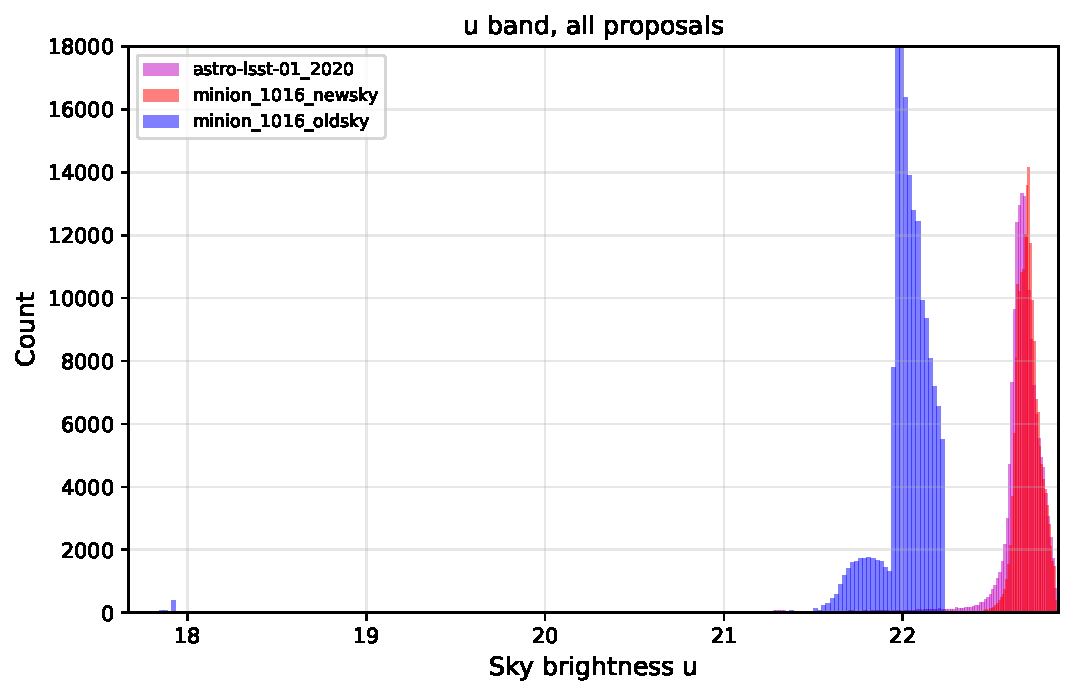
\includegraphics[width=0.3\textwidth]{figures/skybrightness_u_band_ONED_ComboBinnedData}
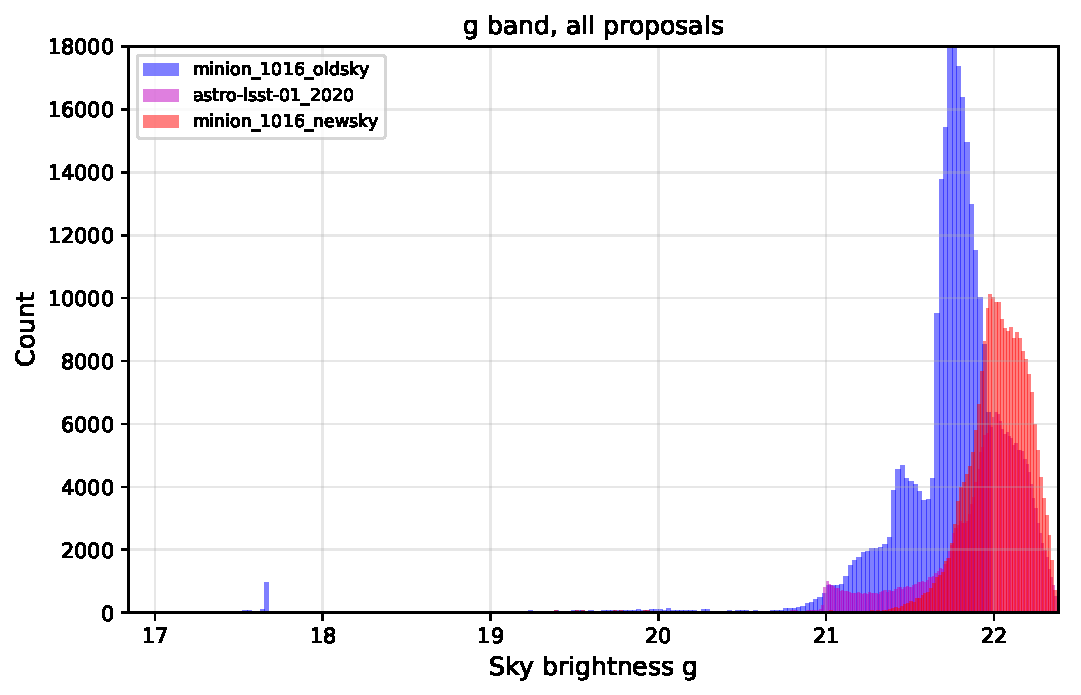
\includegraphics[width=0.3\textwidth]{figures/skybrightness_g_band_ONED_ComboBinnedData}
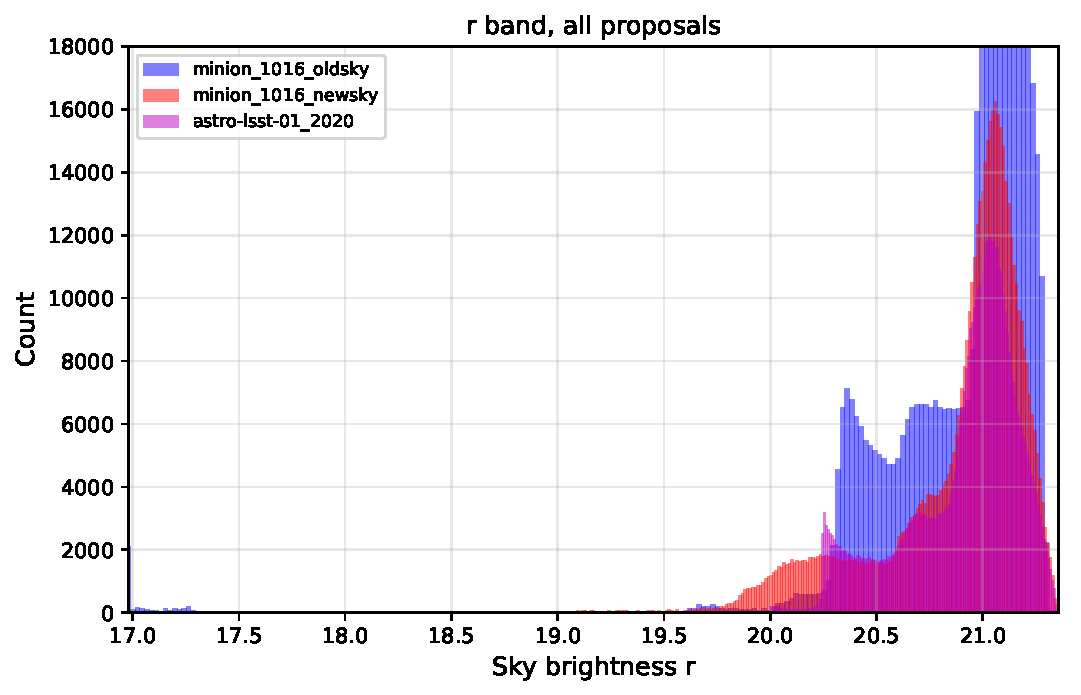
\includegraphics[width=0.3\textwidth]{figures/skybrightness_r_band_ONED_ComboBinnedData} \\
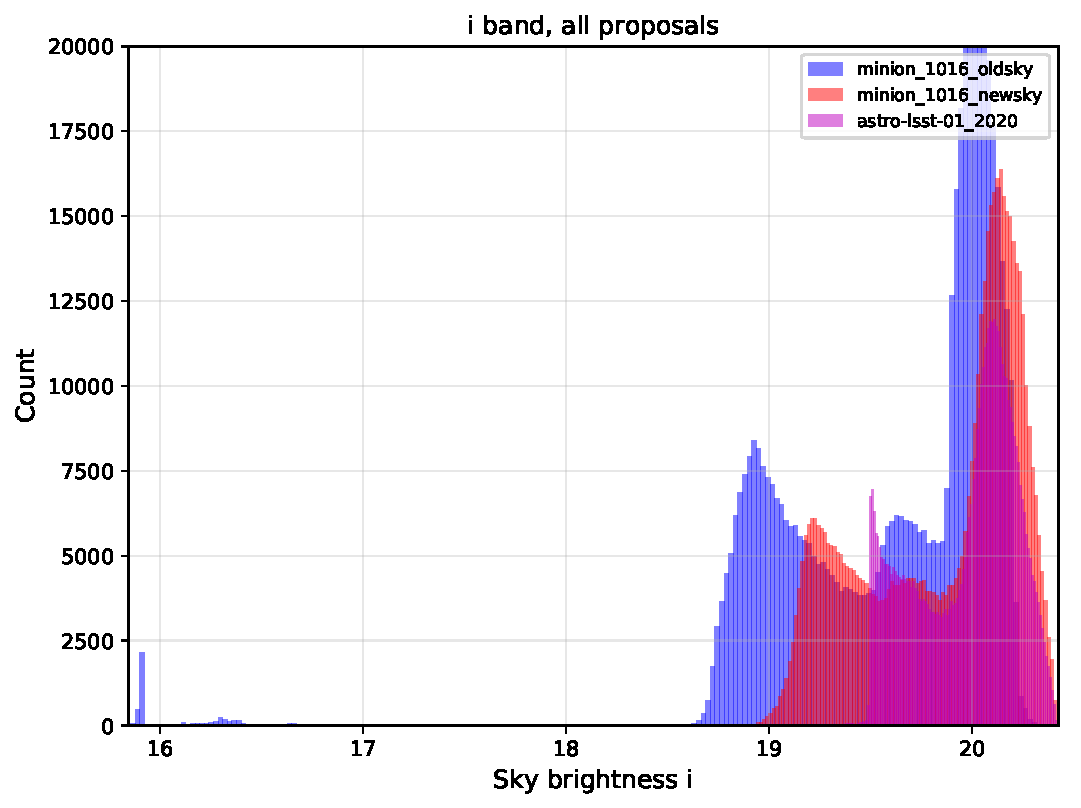
\includegraphics[width=0.3\textwidth]{figures/skybrightness_i_band_ONED_ComboBinnedData}
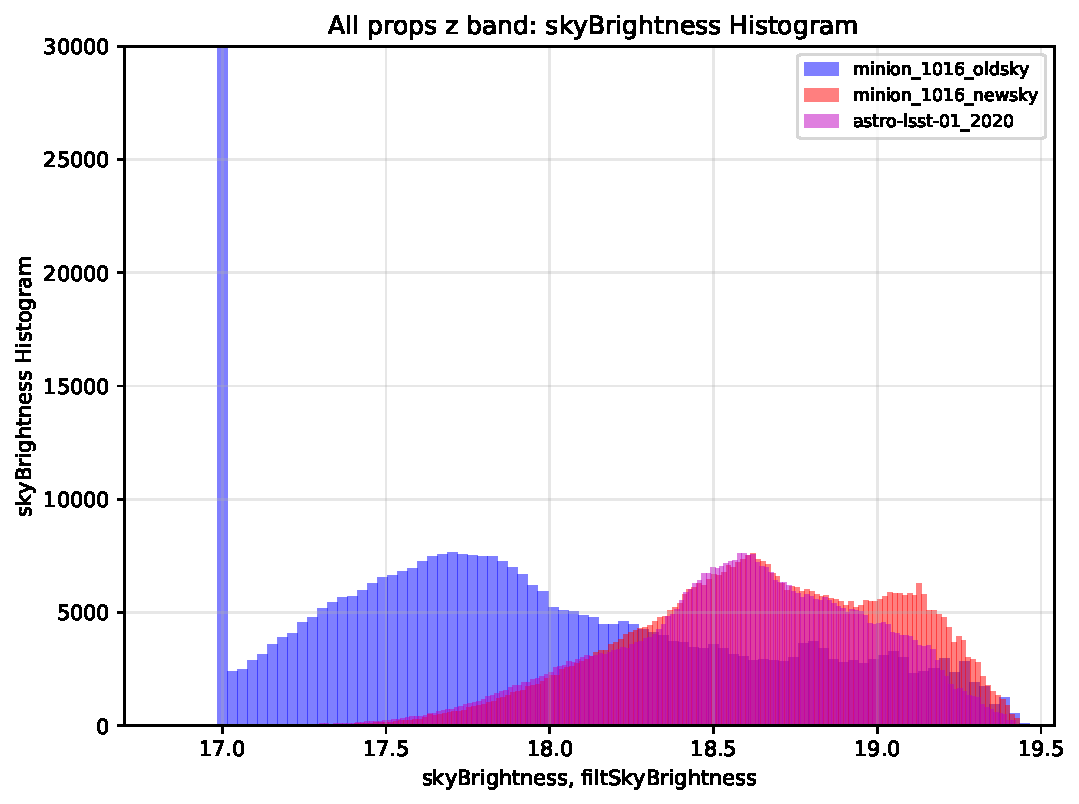
\includegraphics[width=0.3\textwidth]{figures/skybrightness_z_band_ONED_ComboBinnedData}
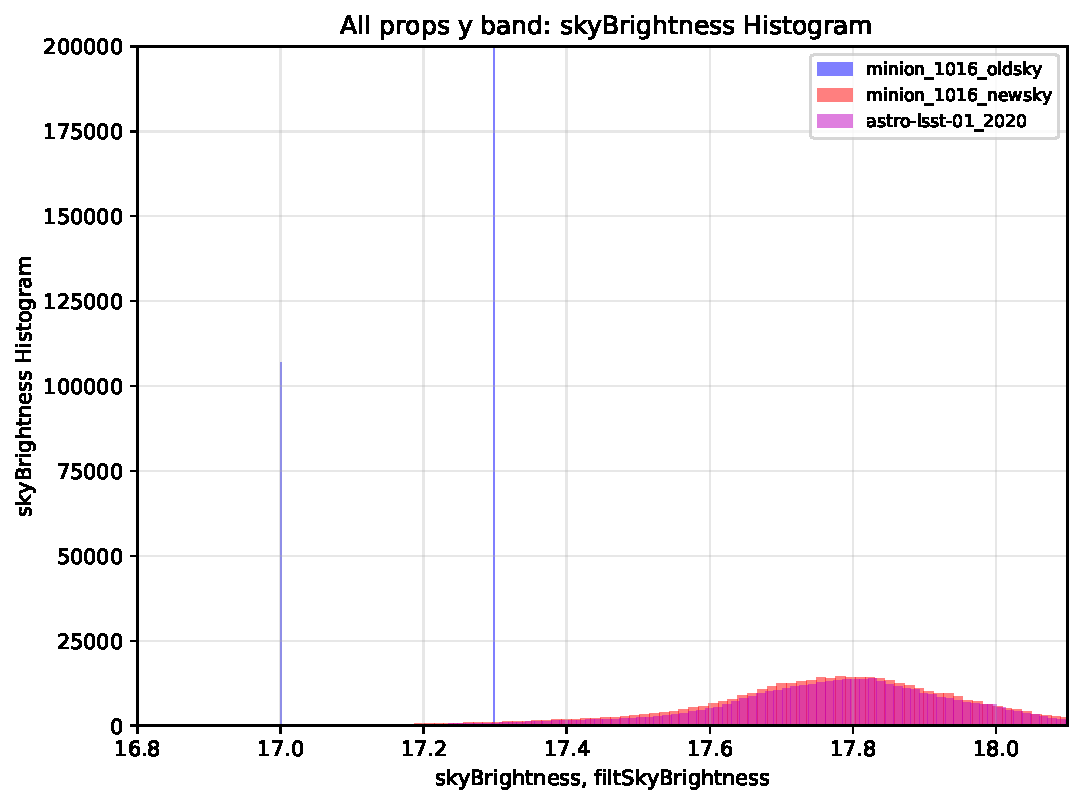
\includegraphics[width=0.3\textwidth]{figures/skybrightness_y_band_ONED_ComboBinnedData}
%\vskip -0.2in
\caption{Sky brightness histograms for minion\_1016 before (minion\_1016\_oldsky) and after (minion\_1016\_newsky) reprocessing with \simsky, and astro-lsst-01\_2020 skybrightness values. The values for astro-lsst-01\_2020 are very similar to the distribution seen in minion\_1016, even though \opsim v4 makes decisions for field pointings based on a knowledge of these skybrightness values in each filter at each pointing, information which was not available for \opsim v3. The changes in skybrightness, and resulting changes in 5$\sigma$ limiting magnitudes, we see due to reprocessing minion\_1016 are thus reasonable to expect in new \opsim v4 runs.
\label{fig:skybrightness}}
\end{figure}

The effect of these decreases in sky brightness are a resulting increase in the 5$\sigma$ limiting depths. There was, however, also an update in the expected throughput of the LSST system after the time of the original minion\_1016 limiting magnitude calculations, and this is also reflected in the change seen in the 5$\sigma$ depths. The throughput changes resulted in an overall decreased sensitivity, an effect which is strongest in the $u$ and $g$ bands. See Table~\ref{tab:m5depth} for the median 5$\sigma$ limiting magnitudes per visit in the WFD observations.

\begin{table}[ht]
\caption{Individual image 5$\sigma$ limiting magnitudes for minion\_1016 before and after reprocessing with \simsky, and astro-lsst-01\_2020. The changes in limiting magnitude correspond to 0.5 times the change in skybrightness, appropriate for the change in SNR, but there were additional changes in the expected throughput of the telescope included in the reprocessing that result in the final m5 changes being slightly smaller than expected.}
\begin{center}
\begin{tabular}{lrrr}
\toprule
{} &  minion\_1016\_oldsky &  minion\_1016\_newsky &  astro-lsst-01\_2020 \\
\midrule
Median m5 WFD u band &           23.137883 &           23.111817 &           23.079406 \\
Median m5 WFD g band &           24.472729 &           24.545191 &           24.474827 \\
Median m5 WFD r band &           24.153684 &           24.085377 &           24.072373 \\
Median m5 WFD i band &           23.392901 &           23.470681 &           23.542878 \\
Median m5 WFD z band &           22.223935 &           22.759990 &           22.720512 \\
Median m5 WFD y band &           21.571697 &           21.800913 &           21.819558 \\
\bottomrule
\end{tabular}
\end{center}
\label{tab:m5depth}
\end{table}

\section{Effect of changing the slew time and filter change cost functions}

The slew time cost function changed slightly between \opsim v3 and v4, substituting an equation that is parametrized by $t_{ref}$, $c_{ref}$, and $t_{max}$, where $t_{ref}$ is intended to be the `reference' slew, $c_{ref}$ is the standard cost of that reference slew, and $t_{max}$ represents the time of a very long slew. The slew time cost function increases rapidly over a range of short slews, and then increases slowly when approaching $t_{max}$.  The cost associated with a range of slew times, with the standard parameters is illustrated in Figure~\ref{fig:slewcost}.  The resulting distribution of slew times in the \opsim v3 baseline, minion\_1016, and the \opsim v4 run with the major new features turned off, astro-lsst-01\_2020, are very similar for short slews, while once into the long slew regime, v4 allows longer slews more often.

\begin{figure}[ht]
\centering
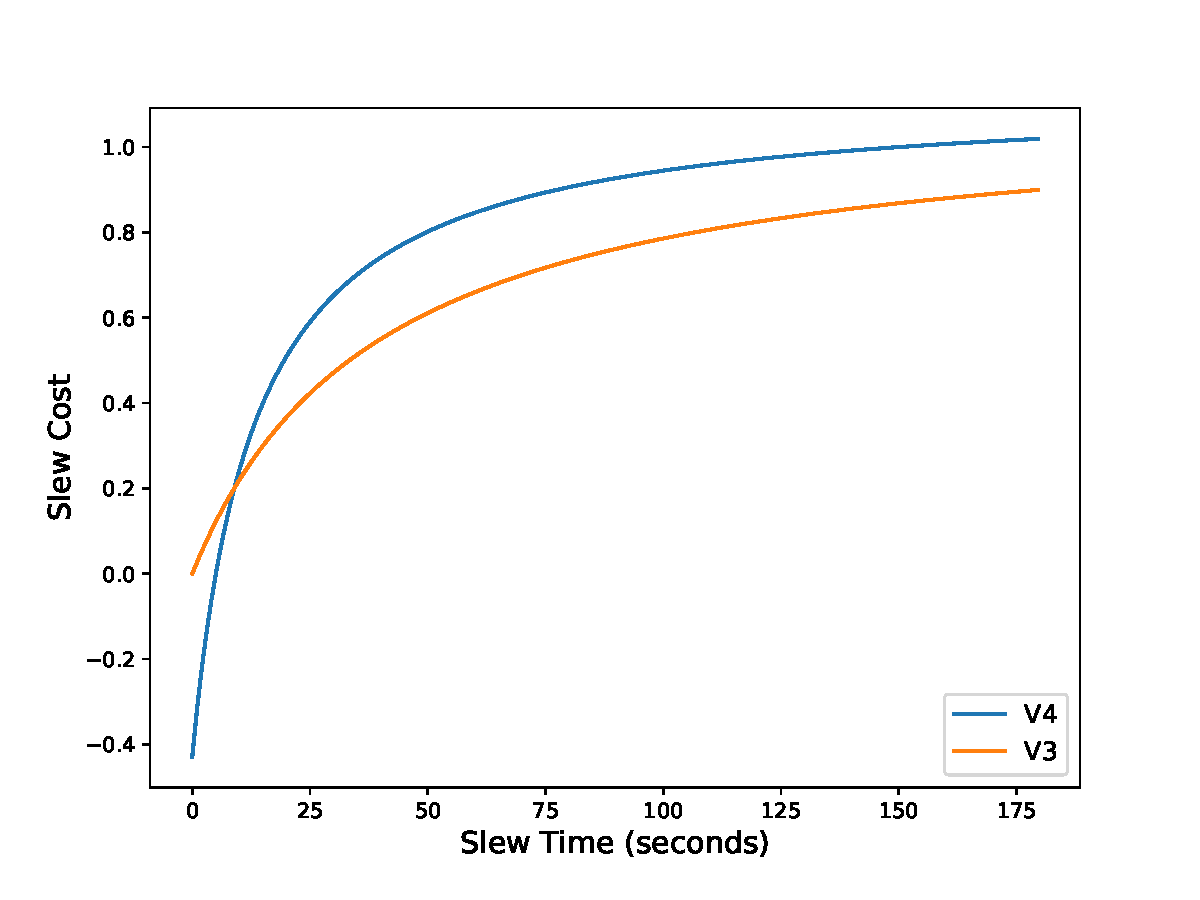
\includegraphics[width=0.37\textwidth]{figures/slewcost}
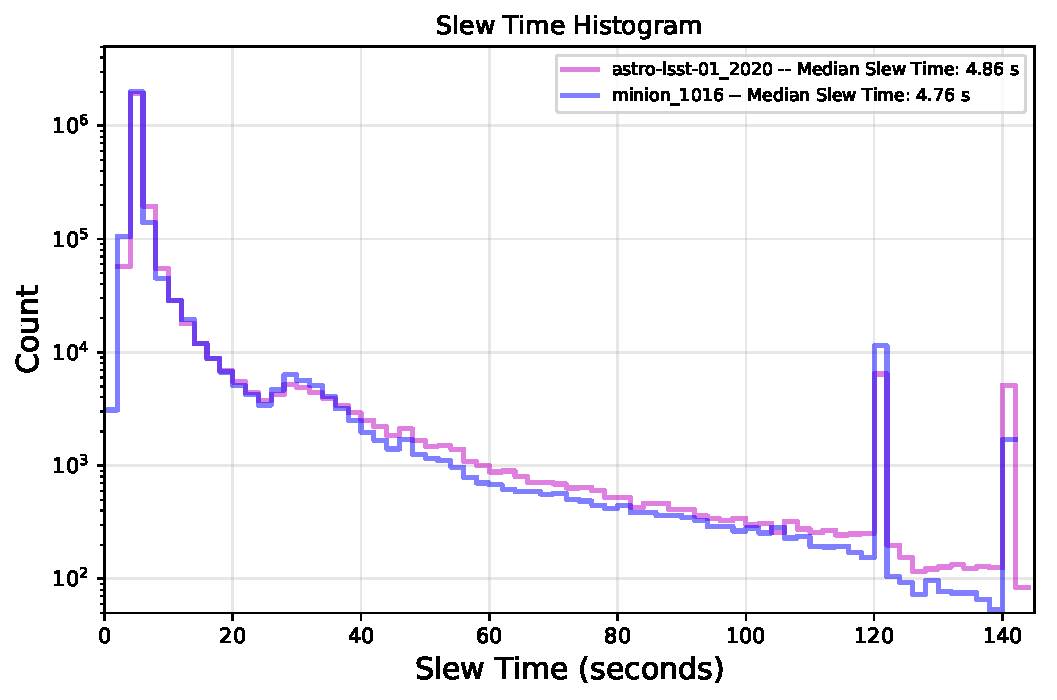
\includegraphics[width=0.4\textwidth]{figures/slewtimes}
\caption{Left: Slew time cost associated with a given slew time, using the default values for $t_{ref}$ (5s), $c_{ref}$ (0.3) and $t_{max}$ (150s). The slew time required is determined by the model of the telescope movement. The cost associated with that slew time is used in the ranking algorithm for choosing the next target in the scheduler. Right: The distribution of slew times in minion\_1016 and astro-lsst-01\_2020 (an \opsim v4 simulation run without new v4 features).
\label{fig:slewcost}}
\end{figure}

The filter change cost calculation was also changed between \opsim v3 and v4, in order to reduce the number of filter changes, particularly on a rapid timescale. The result is that astro-lsst-01\_2020 has 11213 total filter changes, compared to 14194 for minion\_1016; over 20\% fewer filter changes in the new survey. The overall number of filter changes in each of the new simulated surveys is similar; between 10,000 -- 12,000 filter changes over the lifetime of the survey.

\section{The addition of time-balancing}

A significant problem in minion\_1016 was that different proposals within the simulated survey completed their observations at different rates. The proposals which requested fewer total visits than the WFD would reach their requested number of visits before the nominal survey baseline of 10 years, instead of spacing the visits out over time appropriately. \opsim v4 adds the capability to rank targets by the overall progress of each proposal towards its total goal number of visits. This means that the rate of acquiring visits for each proposal remains more uniform over the survey lifetime.

\begin{figure}[ht]
\centering
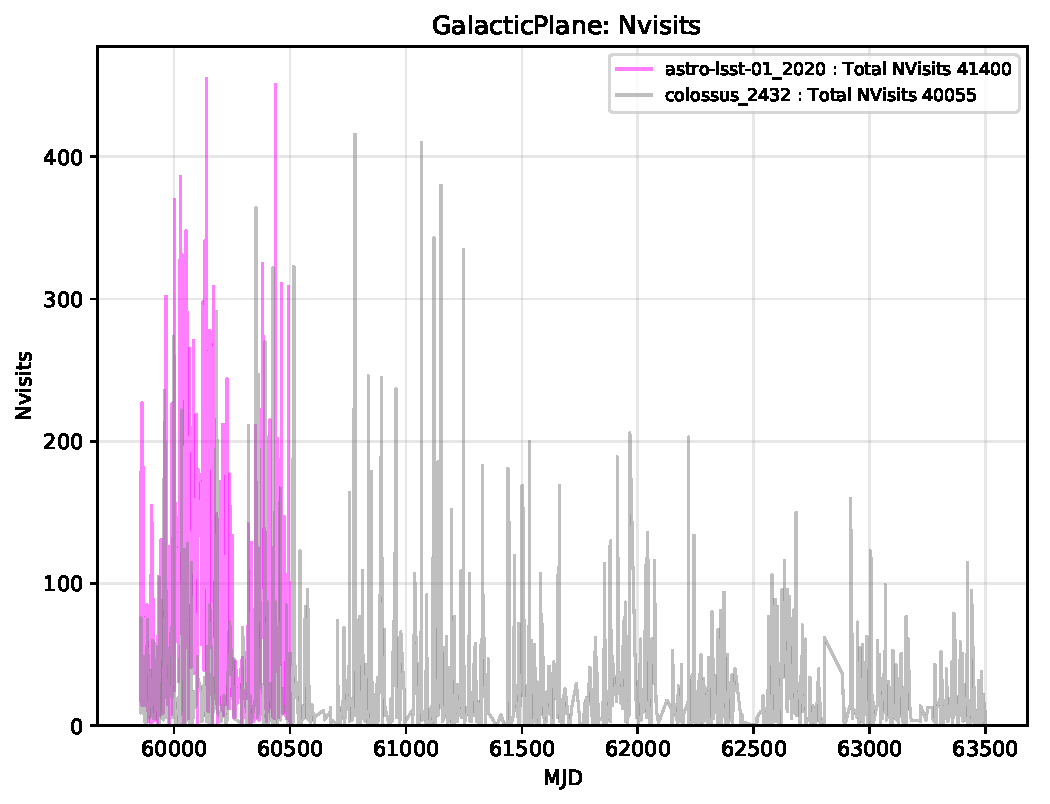
\includegraphics[width=0.3\textwidth]{figures/timebalancing_gp}
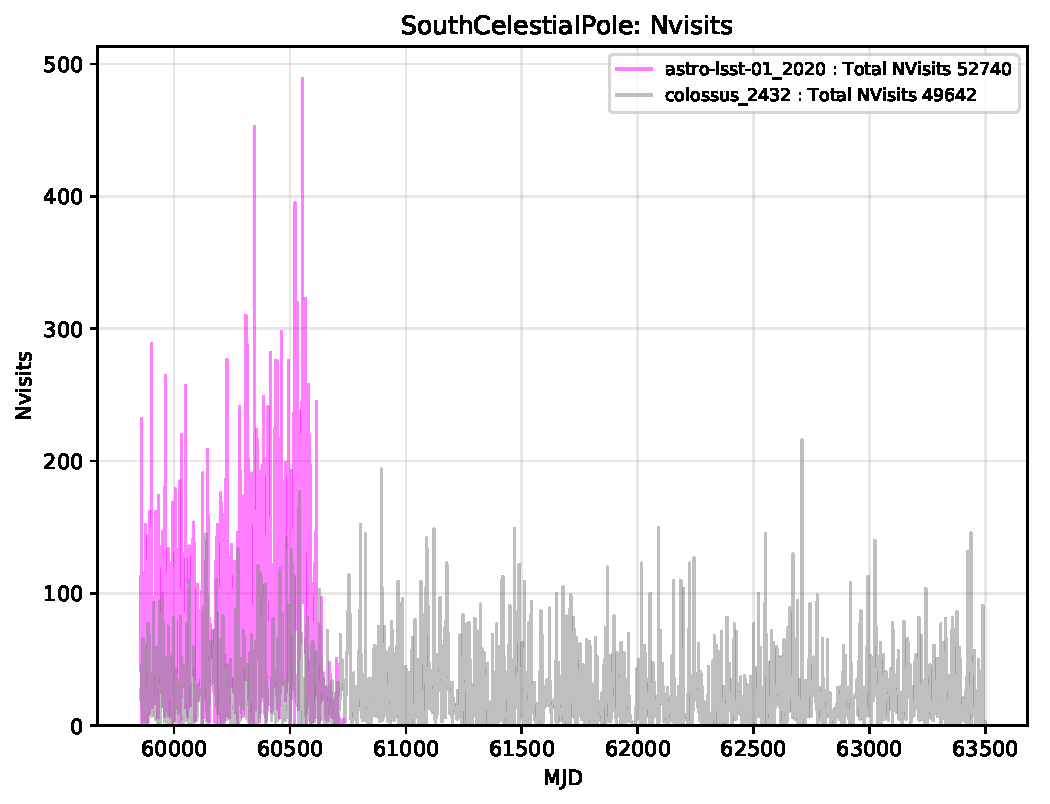
\includegraphics[width=0.3\textwidth]{figures/timebalancing_scp}
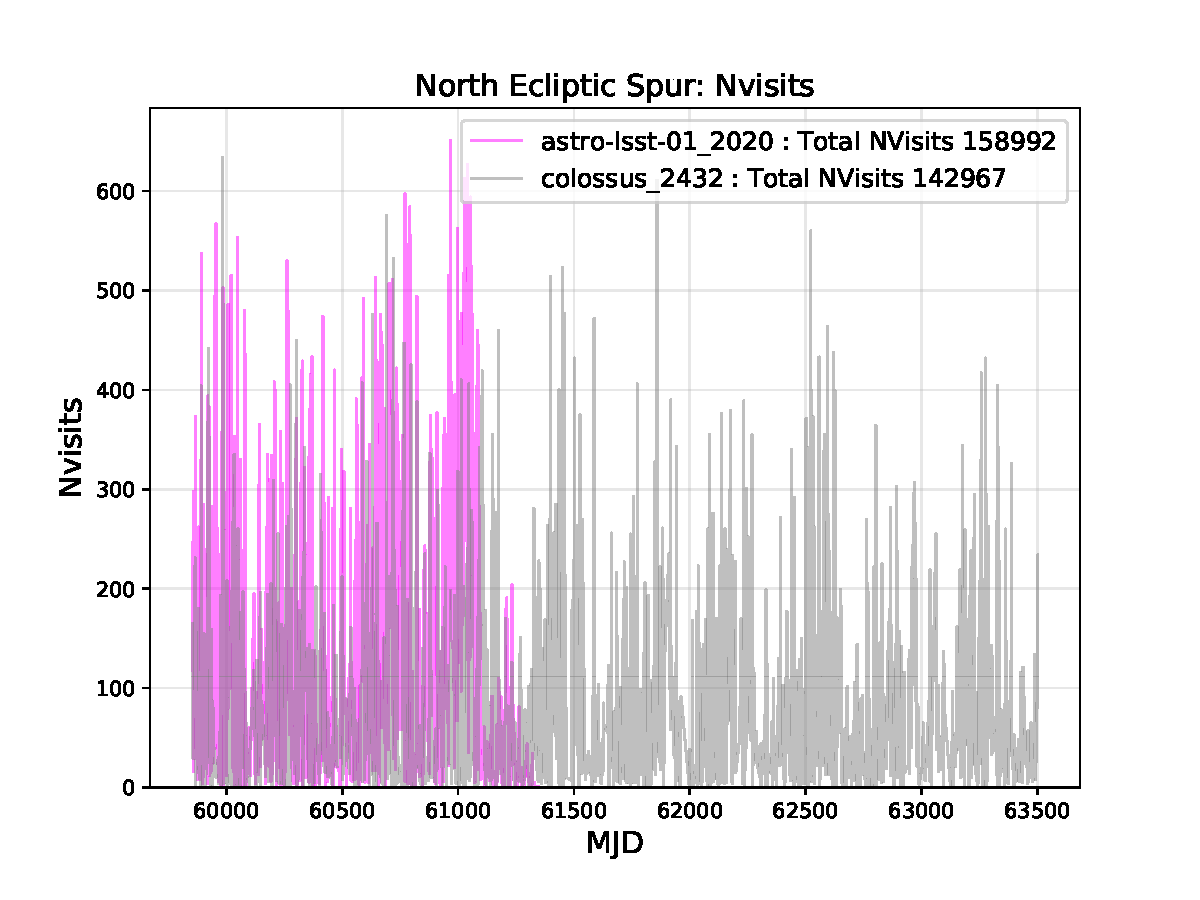
\includegraphics[width=0.3\textwidth]{figures/timebalancing_nes}
\caption{The galactic plane proposal and south celestial pole proposal only request 30 visits per field, per filter. The north ecliptic spur proposal requests about 1/3 of the visits of the full WFD per field. In minion\_1016 and astro-lsst-01\_2020 (an \opsim v4 run without time balancing), these proposals obtained all of their observations only a few years into the survey. With time balancing turned on, the rate of acquiring observations is slower and visits are obtained throughout the simulated lifetime of LSST.
\label{fig:timebalancing}}
\end{figure}


\section{Effect of airmass and HA bonuses}

In a general sense, observations are most effective when obtained as near as possible to the meridian. This is where they have the lowest possible airmass, which results in smaller seeing values. Under dark sky conditions, this is also generally where the faintest sky background is found. Together these effects produce fainter limiting magnitudes near the meridian. In practice, additional considerations such as requirements to return to a field within a night or within a certain range of nights, the presence of the moon or galactic plane, and other constraints mean that observations away from the meridian can also be necessary. In \opsim v3, hard cutoff values for airmass limits were provided, but there was no way to `prefer' observations near the meridian. In \opsim v4, we now have the capability to choose observations that prefer low airmass (via the 'airmass bonus') or low hour angle angle (via the 'hour angle bonus').

The bonus values are implemented as
\begin{eqnarray}
X_{bonus} = X_{bonus\, weight}  \frac {X_{max} - X}{X_{max} - 1}\\
HA_{bonus} = HA_{bonus\, weight}  \left( 1 - \frac{| HA |}{HA_{max}} \right)
\end{eqnarray}
where the bonus weight ($X_{bonus\, weight}$, $HA_{bonus\, weight}$) is the overall weight assigned to the bonus value, a configurable parameter ({\it i.e.} when referring to an airmass bonus of 0.5, the weight is set to 0.5). $X_{max}$ is always set to the maximum airmass allowed for each filter in the proposal, matching the cutoff airmass value. $HA_{max}$ is a configurable parameter for each proposal.

We investigated the effect of each of these bonus parameters, to determine how best to configure the scheduler. We find that including either of these bonus parameters to the scheduler adds some non-uniformity to the resulting sky coverage. When choosing the field for the next visit, the scheduler balances (approximately):
\begin{itemize}
\item the number of visits already obtained at that field, compared to the number of visits obtained for all other fields in the proposal
\item if the field currently needs a return visit (to make a pair within a night)
\item the slew time required to get to that field
\item any bonus value added to that field (the airmass or hour angle bonus).
\end{itemize}
Early in the survey, all fields have approximately the same number of visits and so the bonus values tend to be more important; later in the survey, any previous non-uniformities caused by weather or previous quirks in scheduling tend to be more important. Other sources of non-uniformity include the slew time (which is non-linear due to closed-loop optics correction requirements after elevation changes of 9 degrees) and revisiting fields or observing deep drilling fields.

In Figure~\ref{fig:nvisits_comp_maps}, the results of two comparable `strength' bonus values are shown. At the end of the ten year survey, the final uniformity in sky coverage is generally similar. However, the surveys do not progress with the same degree of uniformity; the airmass bonus, in particular, adds a predictable declination non-uniformity, as observations are preferred near the zenith (rather than just near the meridian). While both surveys suffer from non-uniformity at any given time, the non-uniformity as a result of the hour angle bonus is smaller. Thus we prefer to use the hour angle bonus to bias observations toward the meridian.

\begin{figure}[ht]
\centering
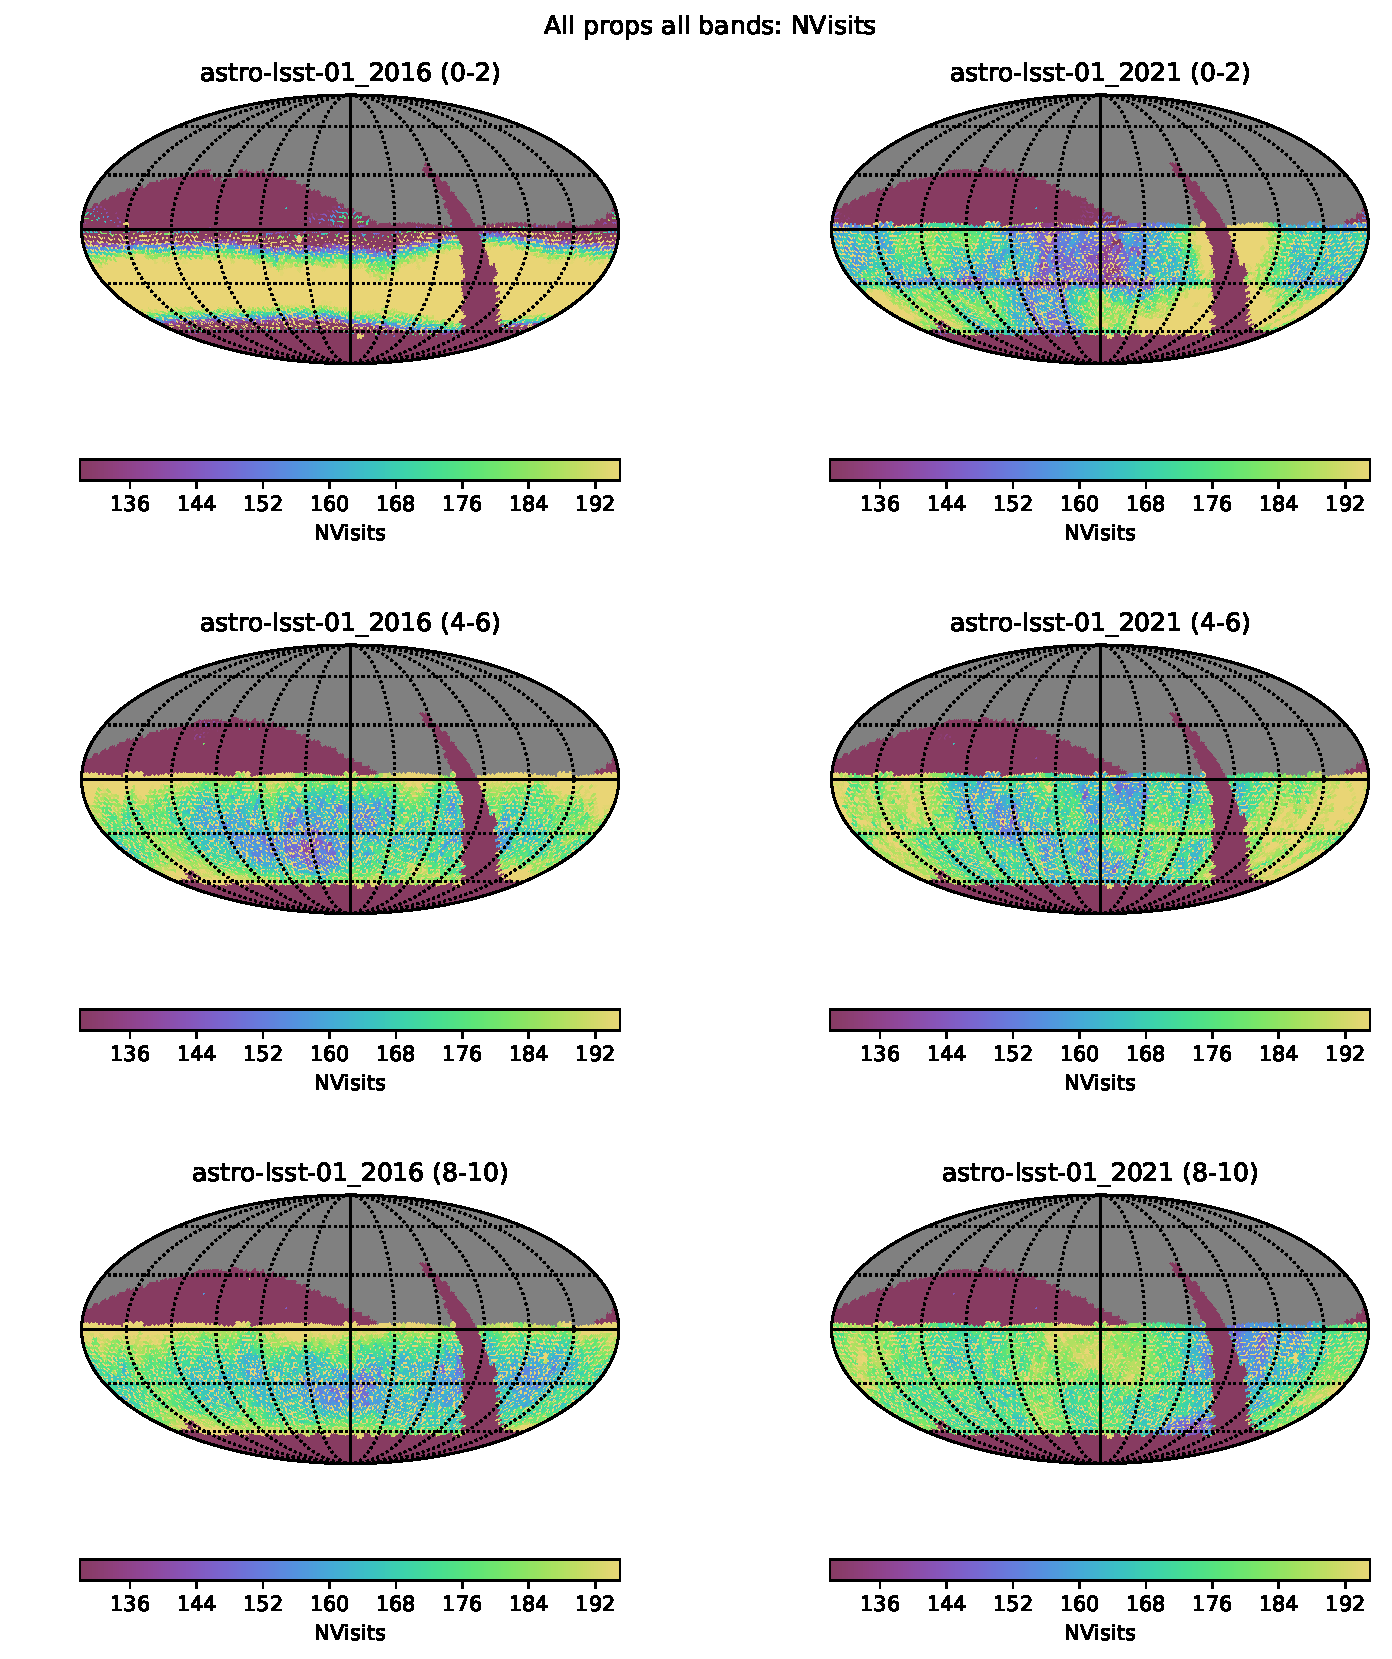
\includegraphics[width=0.7\textwidth]{figures/nvisits_comp_maps}
%\vskip -0.2in
\caption{Comparison of the number of visits in distinct two year time periods throughout the ten year simulated survey lifetime, for two different simulated surveys. In the left column, astro-lsst-01\_2016 is a run with an airmass bonus weight of 0.5 and no $HA$ bonus. In the right columns, astro-lsst-01\_2021 is a run with no airmass bonus but an $HA$ bonus weight of 0.5, with $HA_{max}$ of 6 hours. There is significant non-uniformity with either bonus, however it is a larger effect with the airmass bonus and is, furthermore, strongly tied to the declination of the field.
\label{fig:nvisits_comp_maps}}
\end{figure}


\section{New baseline survey recommendation}

The SRD places requirements on the amount of sky which receives a given minimum number of visits (table 22) and the number of visits over a given minimum area (table 23). Together these specifications are that 18,000 square degrees should receive at least 825 visits (together known as the `fO' metrics). The performance of each of these simulated surveys regarding this important metric is shown in Figure~\ref{fig:srd}. The top panel in the figure illustrates the minimum number of visits an 18,000 sq degree area receives (`Nvisits/825' line) and the amount of area covered which receives at least 825 visits (`Area/18k sq deg' line).  The bottom panel illustrates the changes in the number of visits in each simulated survey, together with the `normalized effective time' of each survey. Effective time is defined as the equivalent amount of on-sky time a survey would require to reach the same total coadded limiting magnitudes assuming all observations were actually taken in a fiducial set of observing conditions; Normalized effective time is this time divided by the actual time spent observing (thus it accounts for differences in the number of days on-sky, if downtime or weather changes between runs). If the simulated observations are obtained in bad conditions (high airmass, bright sky backgrounds), the effective time is smaller; if observations are taken with good conditions, the effective time is larger. We are comparing these values against minion\_1016\_newsky -- the minion\_1016 baseline run, after reprocessing with the \simsky package and recalculated m5 depths using the new throughput values, so that all runs are compared on the same footing.

In the v3 baseline, minion\_1016, the SRD fO metric values were relatively high, as the overall number of visits was larger. With \opsim v4, the airmass or hour angle bonuses add preferences for observations in better conditions (closer to the meridian) but which result in longer slew times. This reduces the overall number of visits but increases the effective time of the survey. The fO metrics fail when these bonuses are set to particularly strong values, primarily because the observations are spread more unevenly over the sky (see Figure~\ref{fig:uniformity_all}.  Observing close to the meridian in some regions of $RA$ is difficult due to the arrangement of the Deep Drilling fields and the North Ecliptic Spur (see Figure~\ref{fig:uniformity_dd}. With a fewer number of overall visits, this pushes some areas down below the benchmark (825 visits) value, causing these fO metric values to fall below the required thresholds.

As discussed in the previous section, we prefer using the HA bonus parameter to achieve better uniformity over time than with the airmass bonus parameter. We also find here that we cannot use a strong HA bonus, due to the resulting non-uniformity in visit distribution across the sky in the WFD fields. We find that the configurations producing astro-lsst-01\_2021 ($HA$ bonus weight = 0.5, $HA_{max}$  = 6 hrs) and astro-lsst-01\_2022 ($HA$ bonus weight=0.3, $HA_{max}$ = 3 hrs) produce reasonable baseline runs; we choose astro-lsst-01\_2022 as the candidate baseline run as it performs slightly better in the effective time metric and produces a slightly smaller number of outliers in the $HA$ distribution.  A comparison of select top-level astro-lsst-01\_2022 statistics versus minion\_1016 is shown in Table~\ref{tab:baseline_comparison}.

Other changes we find with the new baseline run, astro-lsst-01\_2022, when compared with minion\_1016:
\begin{itemize}
\item The non-uniformity of the visit coverage around the sky results in more fields not quite reaching the desired number of visits in all filters (i.e. the MAF `completeness' metric falls). This is undesirable, but given that the SRD requirement on fO is satisfied, this is a place for improvement but not for discarding the simulated survey.
\item The area which receives rapid revisits (revisits between 40 seconds to 30 minutes in time), in particular the area with uniform time coverage within this time span, falls. This is again undesirable, but the minimum amount of area that must be covered within this time frame according to the SRD is still satisfied. In addition, the implementation of this metric should be improved.
\item While the fraction of the total time spent on Deep Drilling remains approximately constant, the number of observations for some of the deep drilling fields fell considerably. The observations for Deep Drilling were not distributed evenly among all fields. This is a place for improvement in the scheduler.
\item Visits are obtained near the meridian, with a much narrower range of hour angle. The western bias in observation is almost nonexistent. See Figure~\ref{fig:hour_angle_comparison}.  This is a positive result, as it also increases the depth in each visit and decreases the seeing. It is linked with the increase in the effective time of the survey.
\item The parallax-DCR degeneracy decreases. This is due to observing near the meridian, thus decreasing DCR signal. This is a positive result.
\item The median value of the maximum gap between visits increases. This implies the season length is (on average) shorter for most fields. At the same time, we see that the median value of the median gap between visits decreases, implying a slightly quicker revisit rate. These two effects are linked, and also tied to observing near the meridian. This is expected to be a positive result in this simulated survey.
\end{itemize}
In short, the implementation of the hour angle bonus in \opsim v4.1.0.10 increases non-uniformity in sky coverage, most likely linked to difficulties scheduling the non-WFD parts of the survey, particularly the deep drilling fields. However, this non-uniformity is balanced by improved conditions due to obtaining observations near the meridian. Visits in the WFD are also obtained over a shorter season each year, but at a more rapid cadence.

\begin{figure}[ht]
\centering
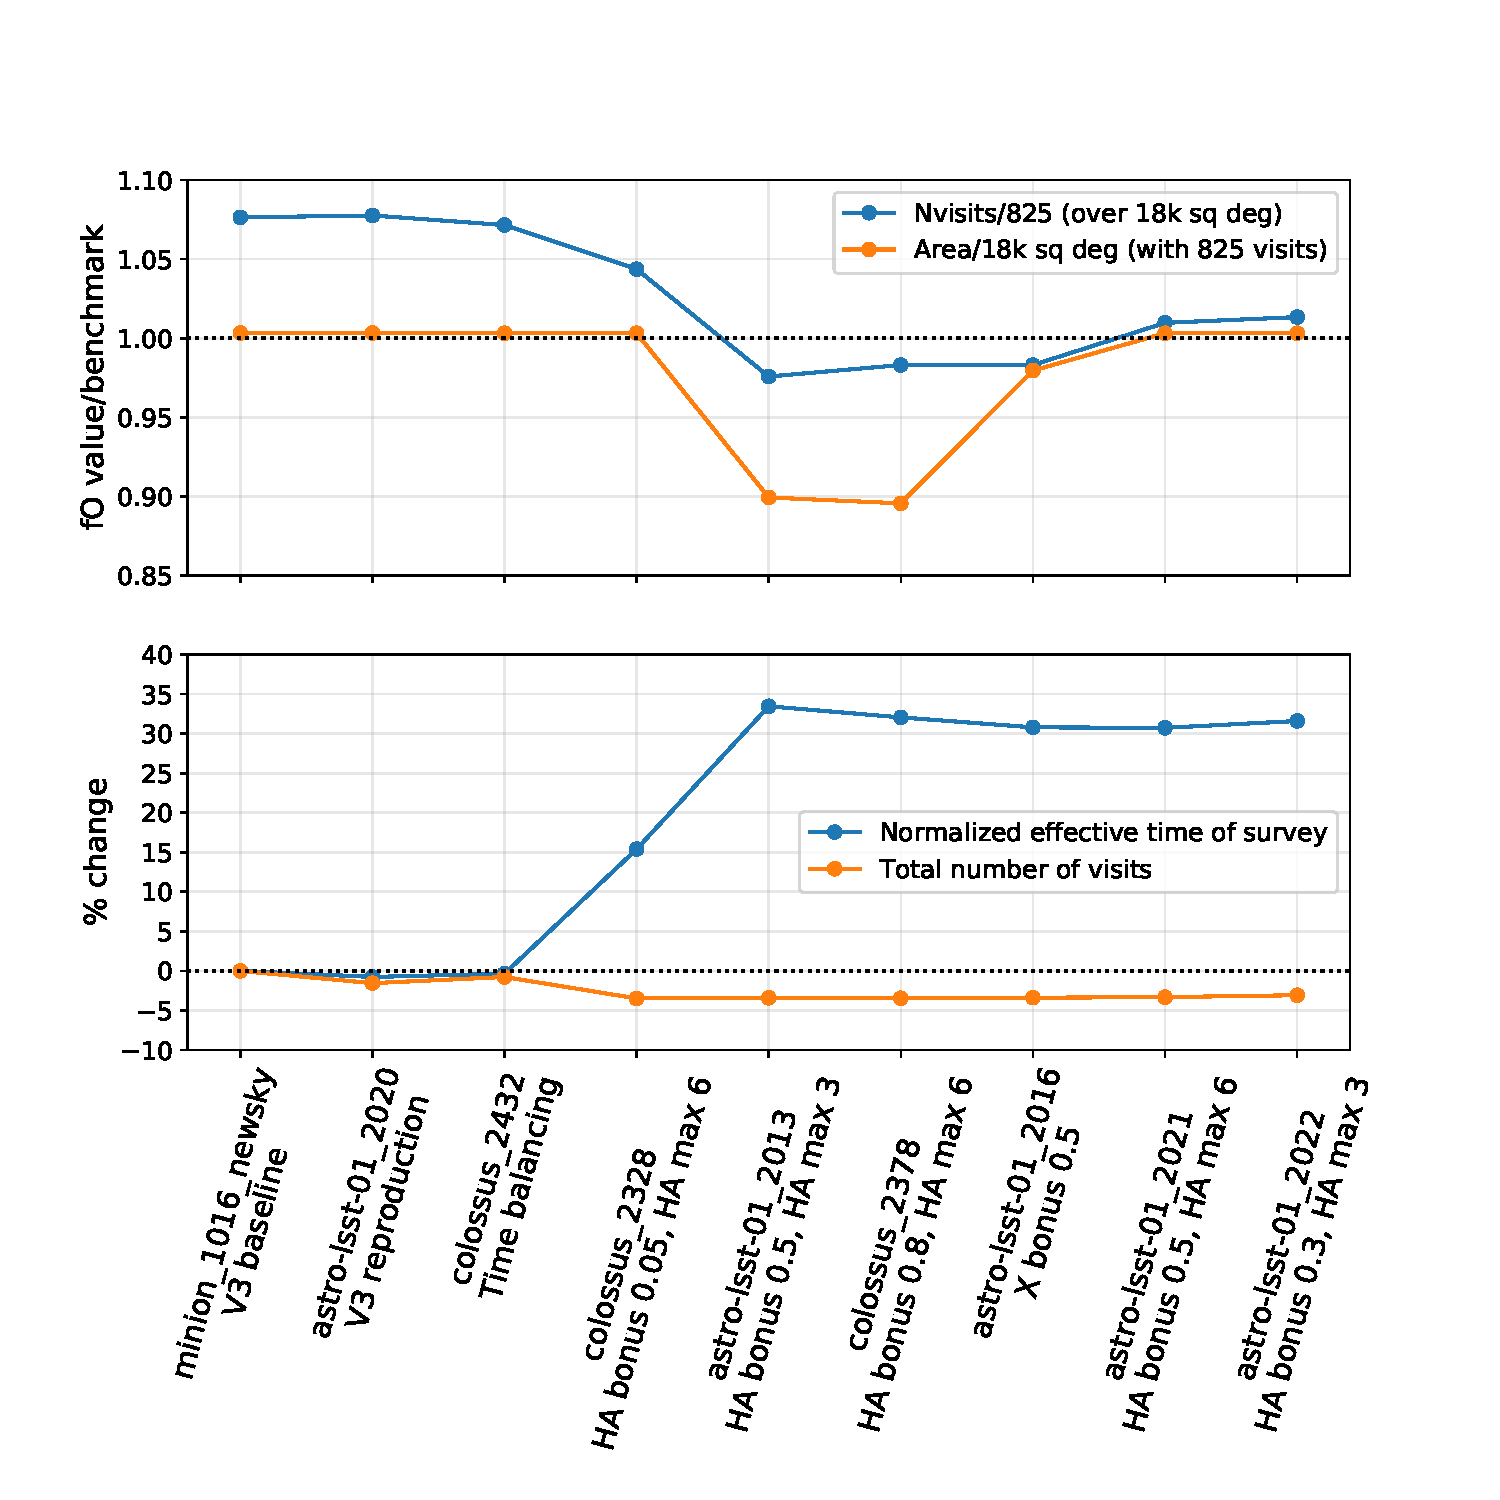
\includegraphics[width=0.9\textwidth]{figures/srd}
%\vskip -0.2in
\caption{The top panel in figure illustrates the minimum number of visits an 18,000 sq degree area receives (Nvisits/825 line) and the amount of area covered which receives at least 825 visits (Area/18k sq deg line).  The bottom panel illustrates the changes in the number of visits in each simulated survey, together with the `normalized effective time' of each survey. Effective time is defined as the equivalent amount of on-sky time a survey would require to reach the same limiting magnitudes as the total coadded depths, assuming all observations were actually taken in a fiducial set of observing conditions. If the actual observations are obtained in bad conditions (high airmass, bright sky backgrounds), the effective time is smaller; if observations are taken with good conditions, the effective time is larger.
\label{fig:srd}}
\end{figure}

\begin{figure}[ht]
\centering
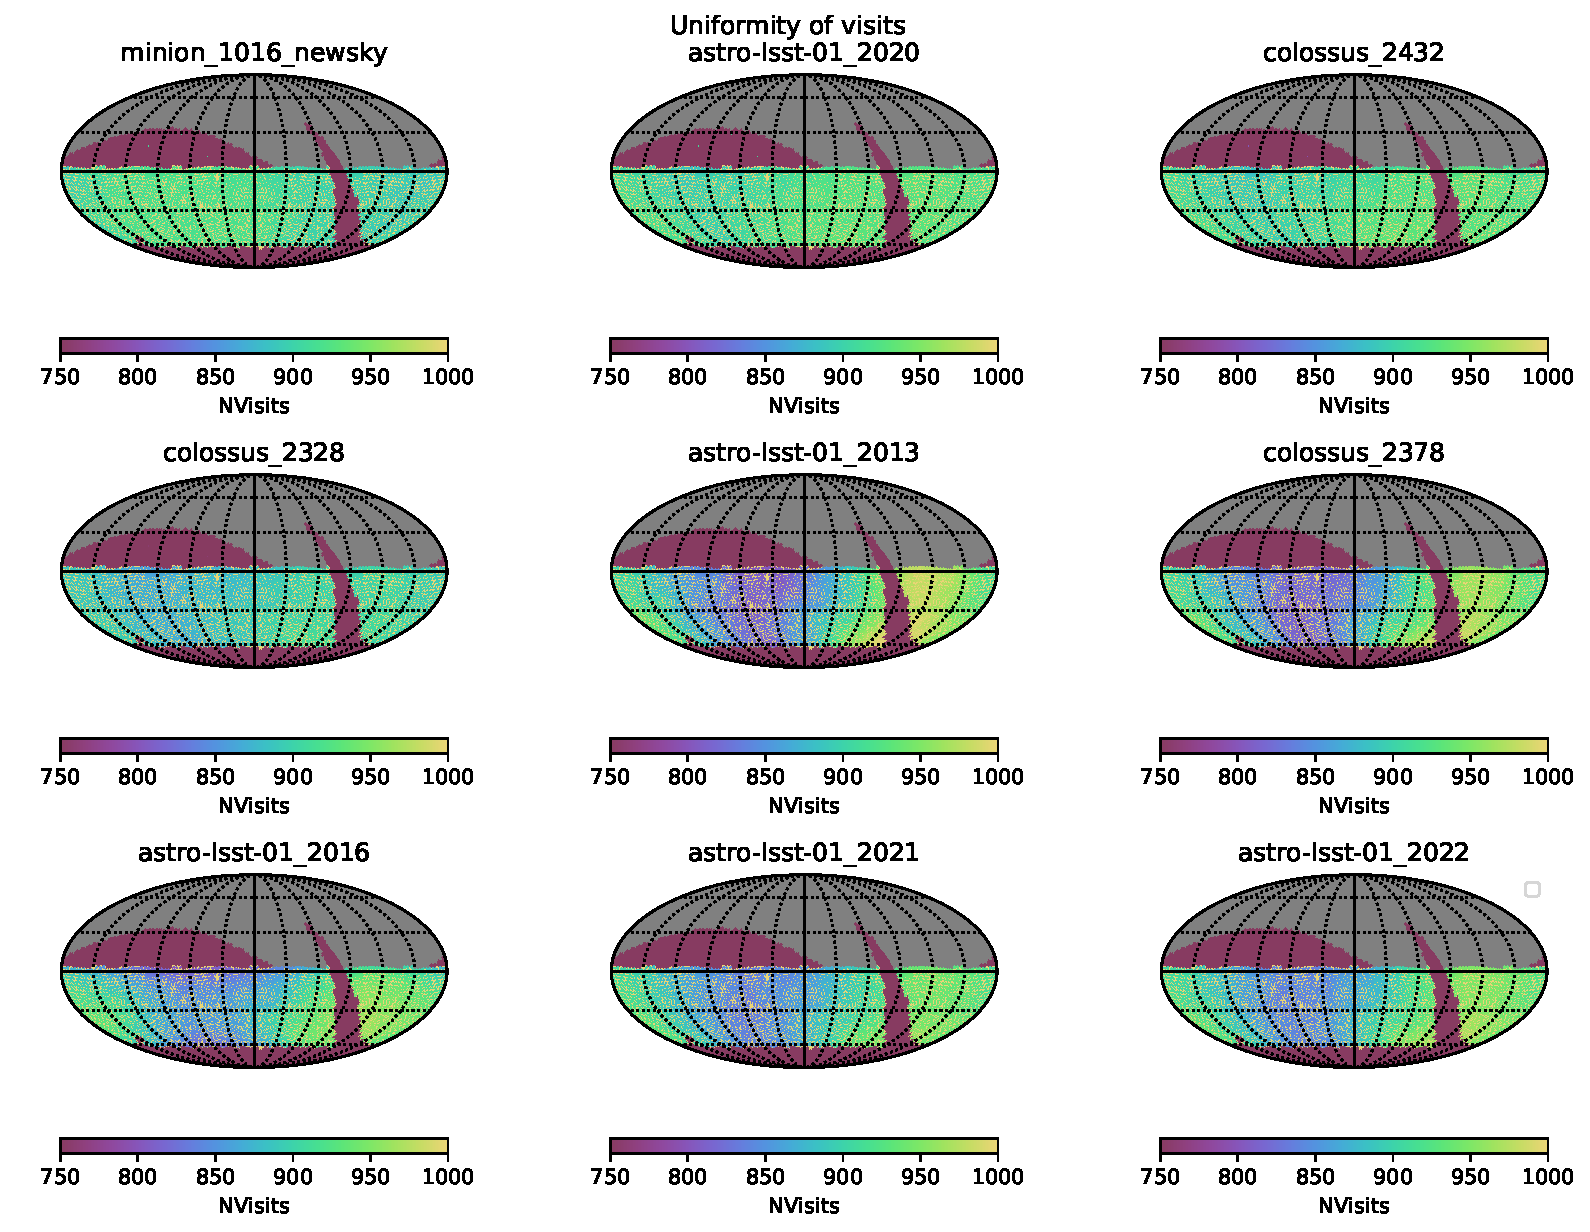
\includegraphics[width=0.9\textwidth]{figures/uniformity_of_visits}
%\vskip -0.2in
\caption{Stronger preferences for observing near the meridian (strong $HA$ bonus coupled with small $HA_{max}$ values) or zenith (strong $X$ bonus) result in more nonuniformity in visits across the WFD. Figure~\ref{fig:uniformity_dd} illustrates that this is correlated to the location of Deep Drilling fields and the location of the North Ecliptic Spur.
\label{fig:uniformity_all}}
\end{figure}

\begin{figure}[ht]
\centering
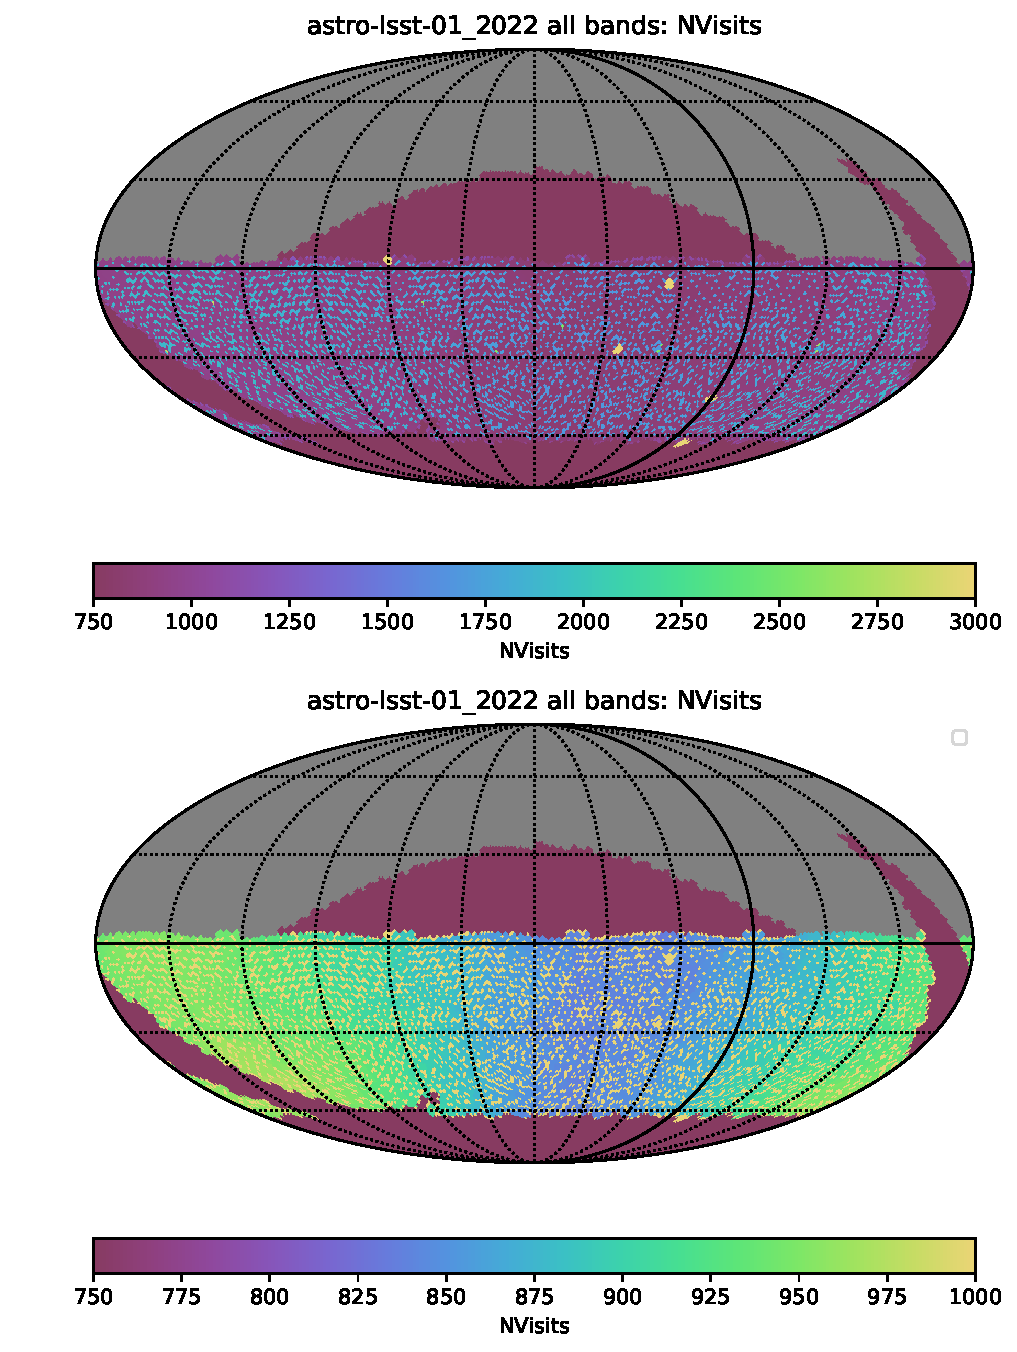
\includegraphics[width=0.6\textwidth]{figures/uniformity_dd}
%\vskip -0.2in
\caption{The nonuniformity in visits, when adding stronger preferences for observing near the meridian, is correlated with the locations of the Deep Drilling fields, four of which are clumped within 30 degrees in $RA$, as well as an increased width of the North Ecliptic Spur. The bottom and top panels show the same information about the number of visits per healpix in astro-lsst-01\_2022, but scaled differently (top to show DD field locations, bottom to show nonuniformity). Improved methods to make the distribution of visits across all ranges of $RA$ more uniform will need to be investigated in future simulated surveys.
\label{fig:uniformity_dd}}
\end{figure}


%\begin{figure}[ht]
%\centering
%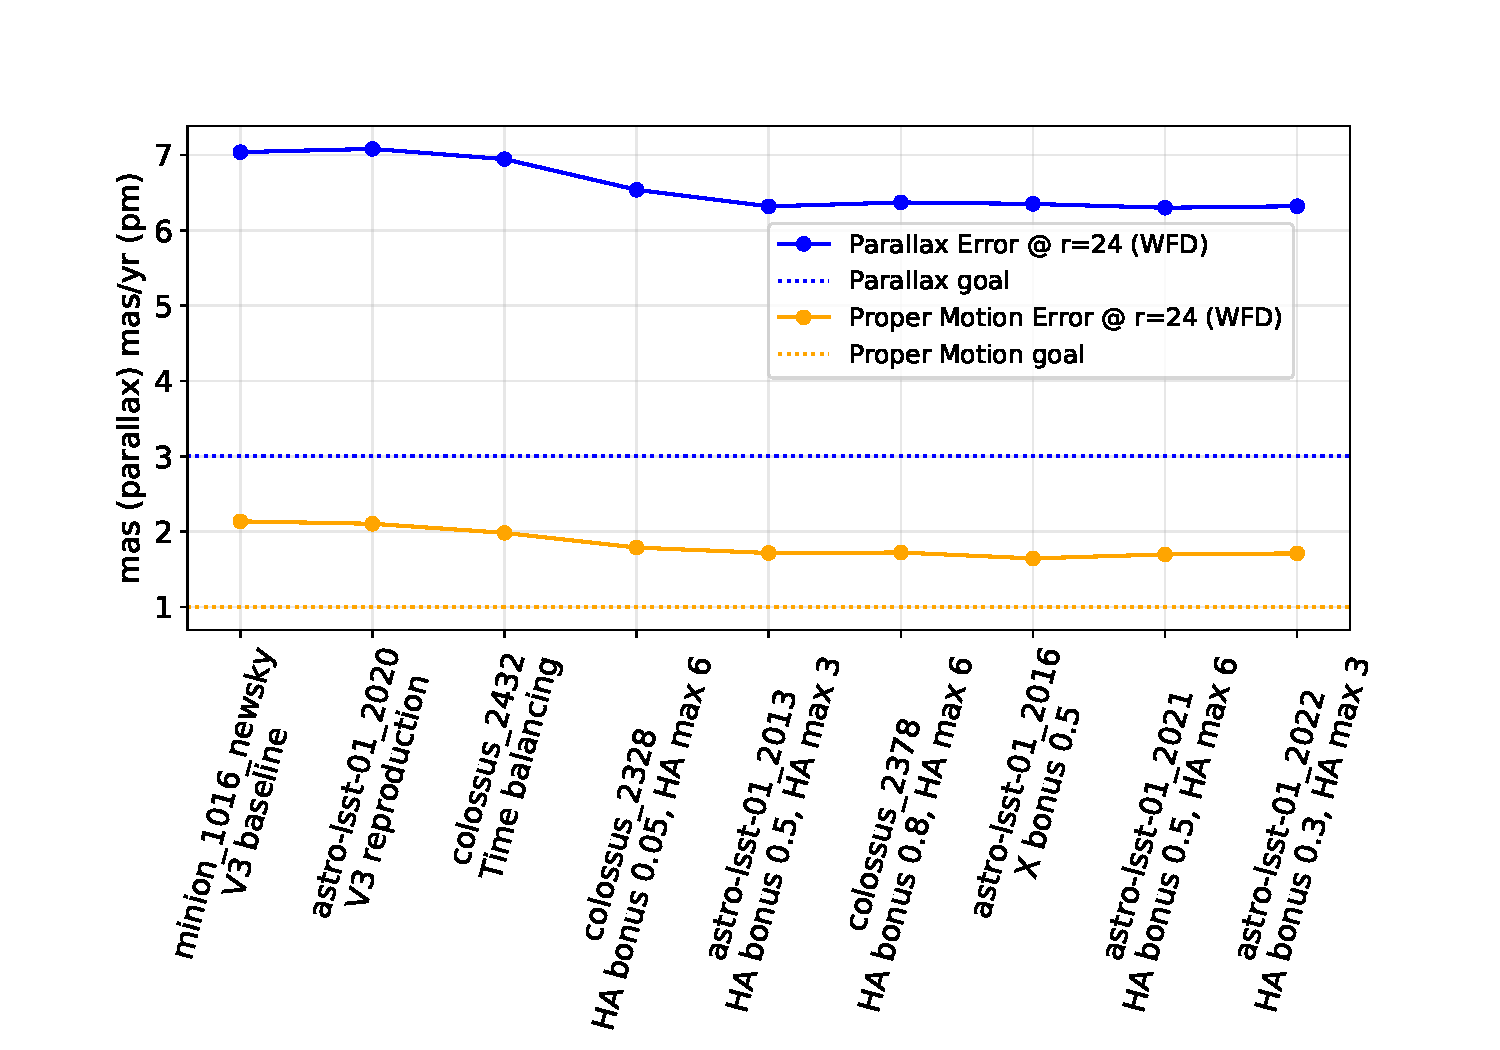
\includegraphics[width=0.9\textwidth]{figures/astrometry}
%\vskip -0.2in
%\caption{
%\label{fig:astrometry}}
%\end{figure}

\begin{table}
\caption{Comparison of select metrics from the \opsim v3 baseline run minion\_1016 and the \opsim v4 suggested baseline run update astro-lsst-01\_2022.}
\small
\begin{center}
\begin{tabular}{lrrr}
\toprule
{} &  minion\_1016\_newsky &  astro-lsst-01\_2022 &  Change (\%) \\
\midrule
fO(18k sq deg): Nvisits/825   &               1.076 &               1.013 &         -6 \\
fO(825): Area/18k sq deg     &               1.003 &               1.003 &          0 \\
Normalized Teff                                    &               0.424 &               0.558 &         32 \\
Total Number of Exposures                                &             2447931 &             2372700 &         -3 \\
Fraction of total visits in WFD                      &               0.851 &               0.864 &          1 \\
Mean Visits Per Night                   &             808.966 &             784.364 &         -3 \\
Median NVisits WFD u band HealpixSlicer            &                  63 &                  62 &         -2 \\
Median NVisits WFD g band HealpixSlicer            &                  88 &                  87 &         -1 \\
Median NVisits WFD r band HealpixSlicer            &                 201 &                 200 &          0 \\
Median NVisits WFD i band HealpixSlicer            &                 202 &                 199 &         -1 \\
Median NVisits WFD z band HealpixSlicer            &                 180 &                 183 &          2 \\
Median NVisits WFD y band HealpixSlicer            &                 181 &                 182 &          1 \\
Median NVisits WFD all bands HealpixSlicer         &                 916 &                 912 &          0 \\
Median CoaddM5 WFD u band HealpixSlicer            &              25.440 &              25.615 &          1 \\
Median CoaddM5 WFD g band HealpixSlicer            &              27.051 &              27.110 &          0 \\
Median CoaddM5 WFD r band HealpixSlicer            &              27.028 &              27.188 &          1 \\
Median CoaddM5 WFD i band HealpixSlicer            &              26.432 &              26.613 &          1 \\
Median CoaddM5 WFD z band HealpixSlicer            &              25.660 &              25.707 &          0 \\
Median CoaddM5 WFD y band HealpixSlicer            &              24.695 &              24.892 &          1 \\
Median Parallax @ 20.0 WFD HealpixSlicer           &               0.535 &               0.551 &          3 \\
Median Parallax @ 24.0 WFD HealpixSlicer           &               7.038 &               6.320 &        -10 \\
Median Proper Motion @ 20.0 WFD HealpixSlicer      &               0.162 &               0.149 &         -8 \\
Median Proper Motion @ 24.0 WFD HealpixSlicer      &               2.138 &               1.713 &        -20 \\
Area (sq deg) with > 800 visits within 30 minutes &            6388.932 &            5834.756 &         -9 \\
Median Fraction of visits in pairs (15-60 min) in gri &               0.909 &               0.895 &         -2 \\
Median value of Median Internight Gap (per healpix)  &               2.950 &               1.973 &        -33 \\
Median seeingFWHMEff WFD r band                        &               0.912 &               0.853 &         -6 \\
Median slewTime All visits                         &               4.756 &               5.175 &          9 \\
Total Number of Filter Changes                    &               14194 &               10644 &        -25 \\
Open Shutter Fraction                                &               0.735 &               0.716 &         -3 \\
\bottomrule
\end{tabular}
\end{center}
\label{tab:baseline_comparison}
\end{table}

\begin{figure}[ht]
\centering
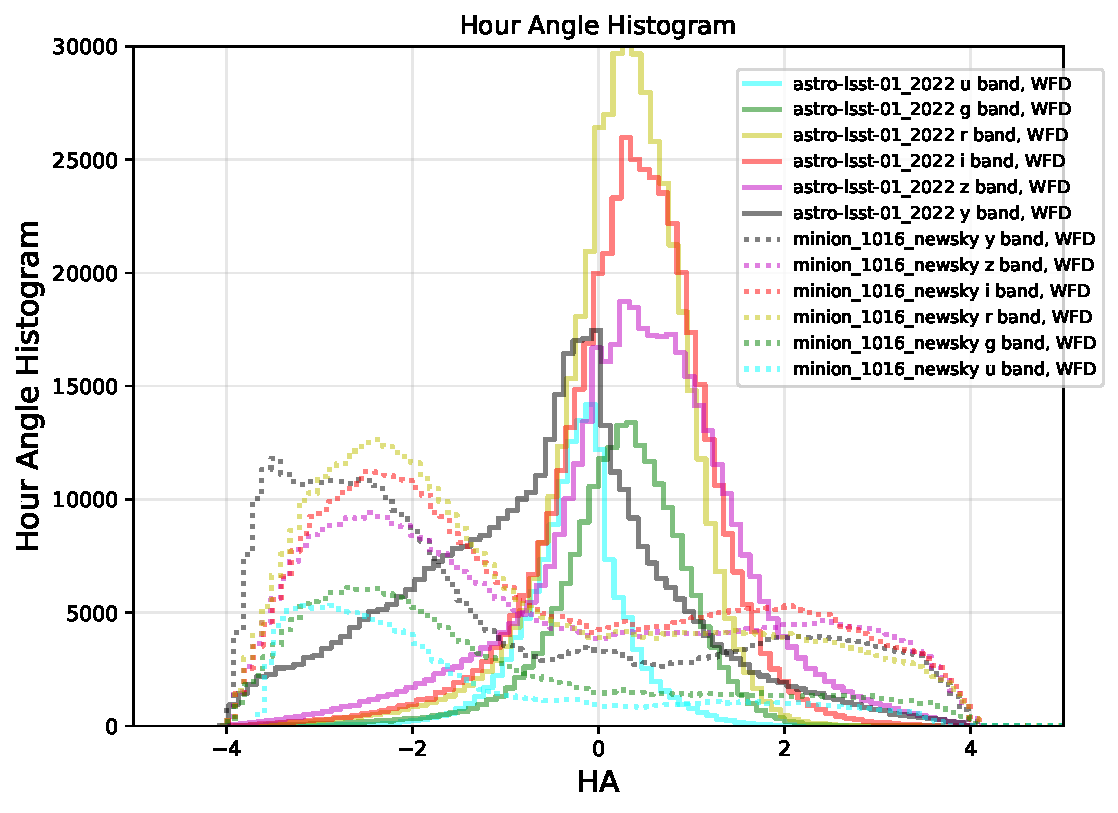
\includegraphics[width=0.8\textwidth]{figures/hour_angle_comparison}
%\vskip -0.2in
\caption{Comparison of the hour angle distribution, per filter, in minion\_1016 (dotted lines) and astro-lsst-01\_2022 (solid lines). The known issue with western bias in minion\_1016 can clearly be seen. This does not occur in astro-lsst-01\_2022, which also has a much tighter distribution of hour angles.
\label{fig:hour_angle_comparison}}
\end{figure}

\begin{figure}[ht]
\centering
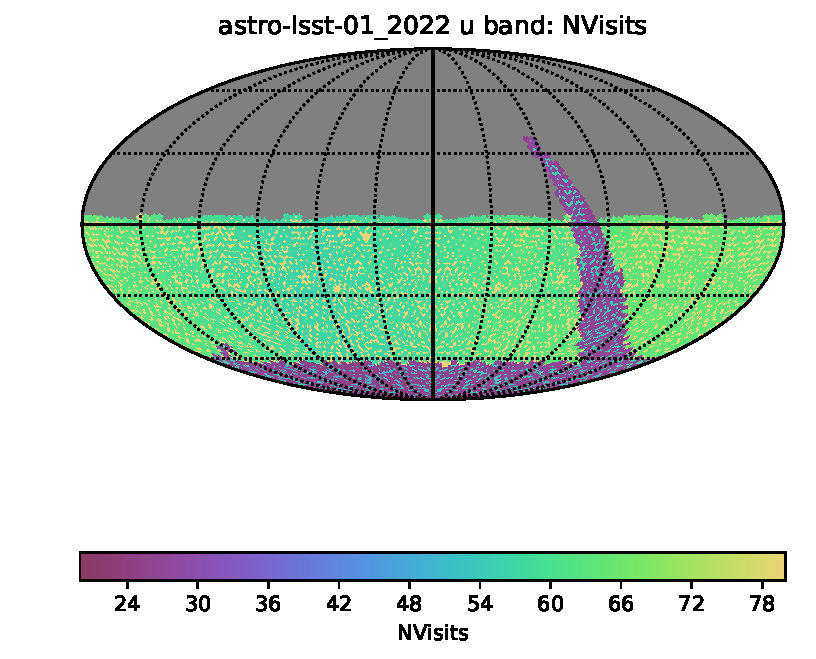
\includegraphics[width=0.4\textwidth]{figures/astro-lsst-01_2022_NVisits_u_band_HEAL_SkyMap}
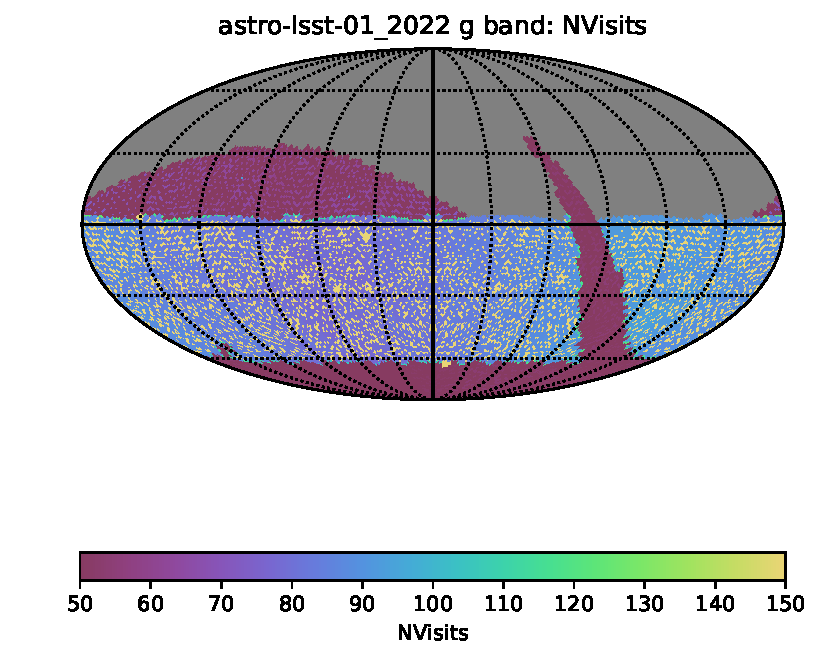
\includegraphics[width=0.4\textwidth]{figures/astro-lsst-01_2022_NVisits_g_band_HEAL_SkyMap} \\
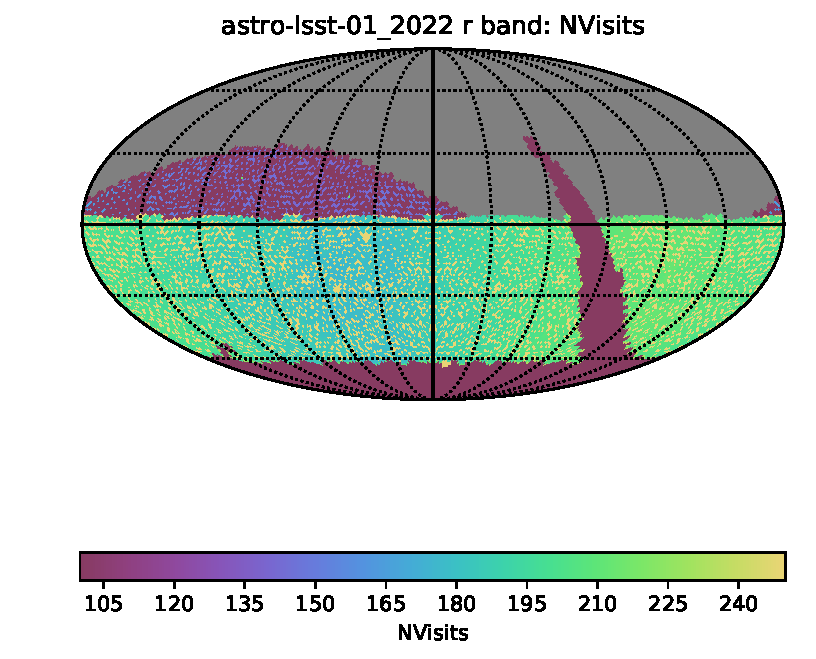
\includegraphics[width=0.4\textwidth]{figures/astro-lsst-01_2022_NVisits_r_band_HEAL_SkyMap}
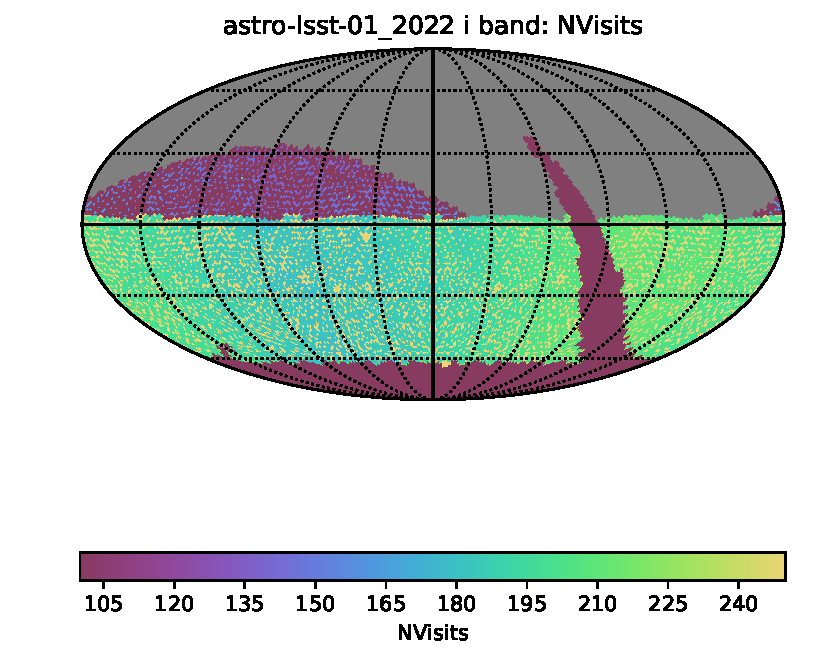
\includegraphics[width=0.4\textwidth]{figures/astro-lsst-01_2022_NVisits_i_band_HEAL_SkyMap} \\
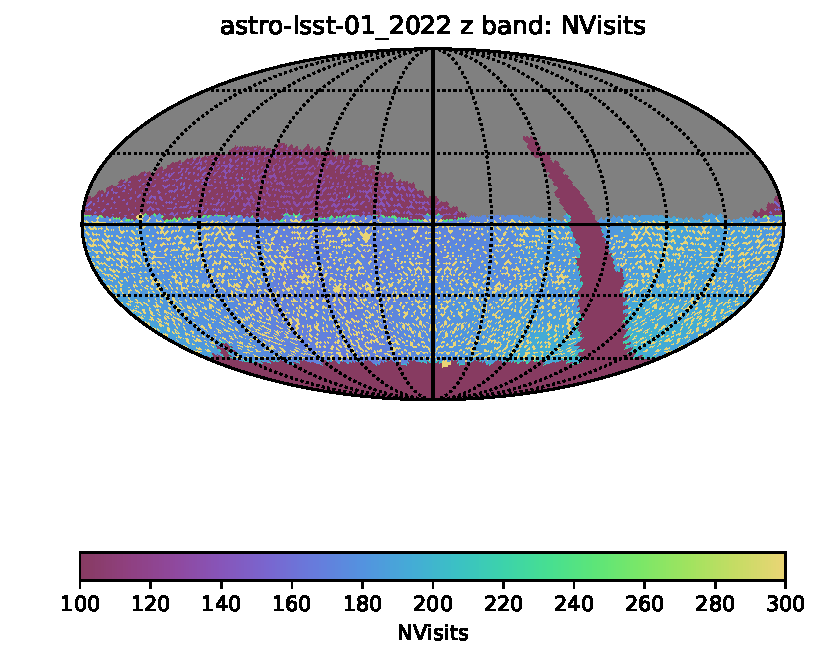
\includegraphics[width=0.4\textwidth]{figures/astro-lsst-01_2022_NVisits_z_band_HEAL_SkyMap}
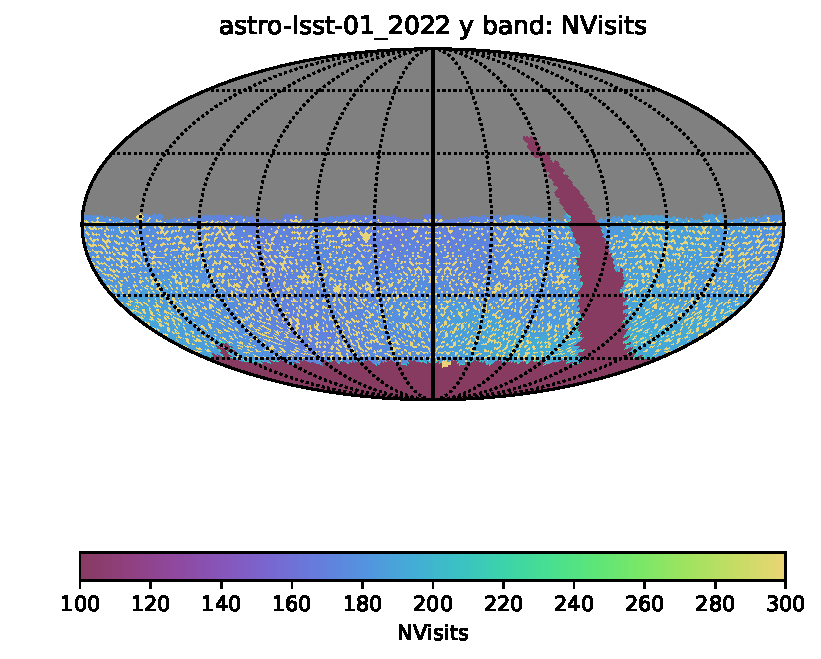
\includegraphics[width=0.4\textwidth]{figures/astro-lsst-01_2022_NVisits_y_band_HEAL_SkyMap}
\caption{Number of visits per filter for astro-lsst-01\_2022.
\label{fig:baseline_nvisits}}
\end{figure}

\begin{figure}[ht]
\centering
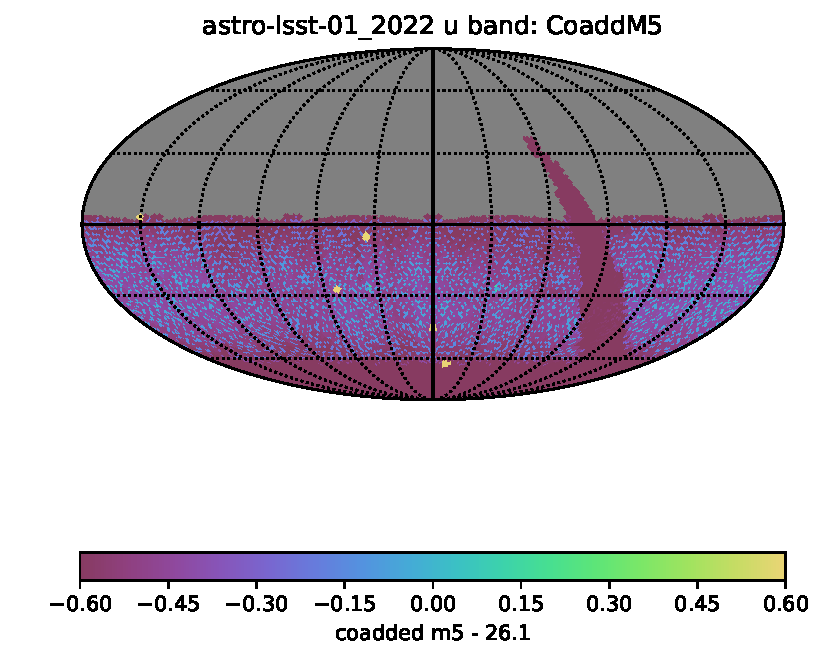
\includegraphics[width=0.4\textwidth]{figures/astro-lsst-01_2022_CoaddM5_u_band_HEAL_SkyMap}
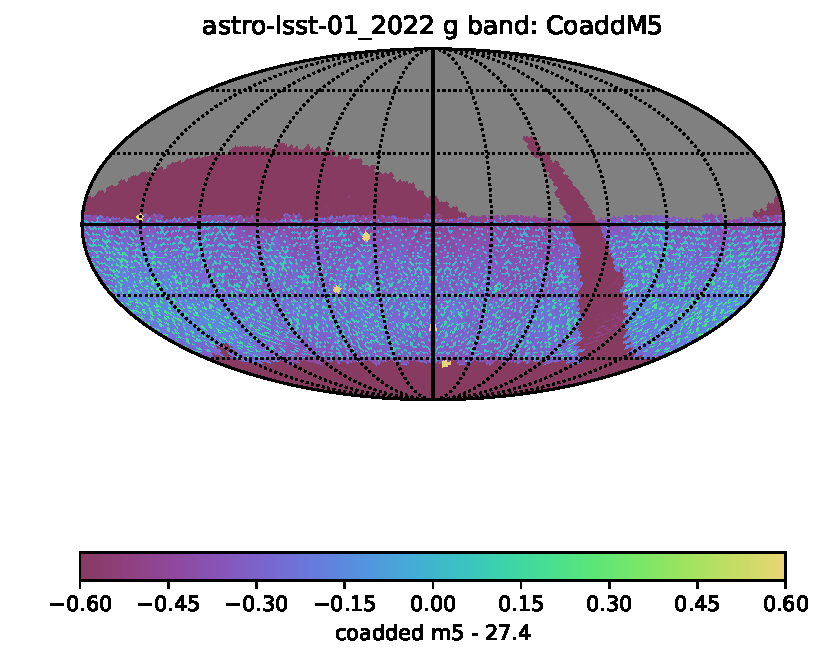
\includegraphics[width=0.4\textwidth]{figures/astro-lsst-01_2022_CoaddM5_g_band_HEAL_SkyMap} \\
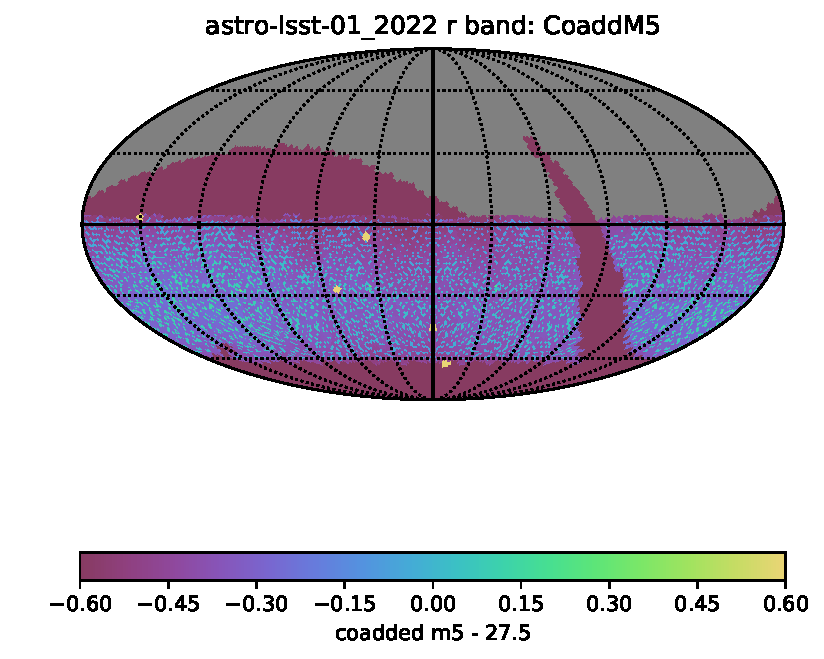
\includegraphics[width=0.4\textwidth]{figures/astro-lsst-01_2022_CoaddM5_r_band_HEAL_SkyMap}
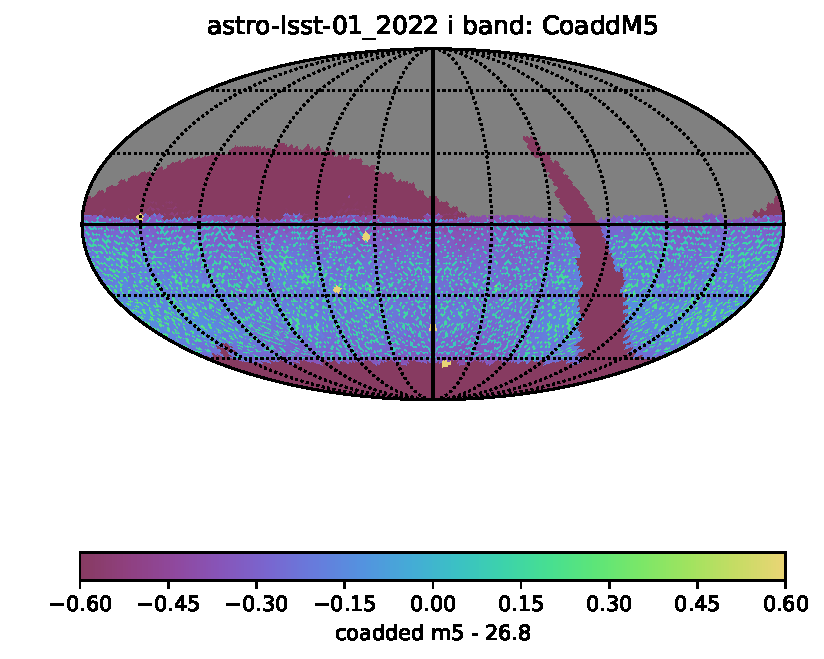
\includegraphics[width=0.4\textwidth]{figures/astro-lsst-01_2022_CoaddM5_i_band_HEAL_SkyMap}  \\
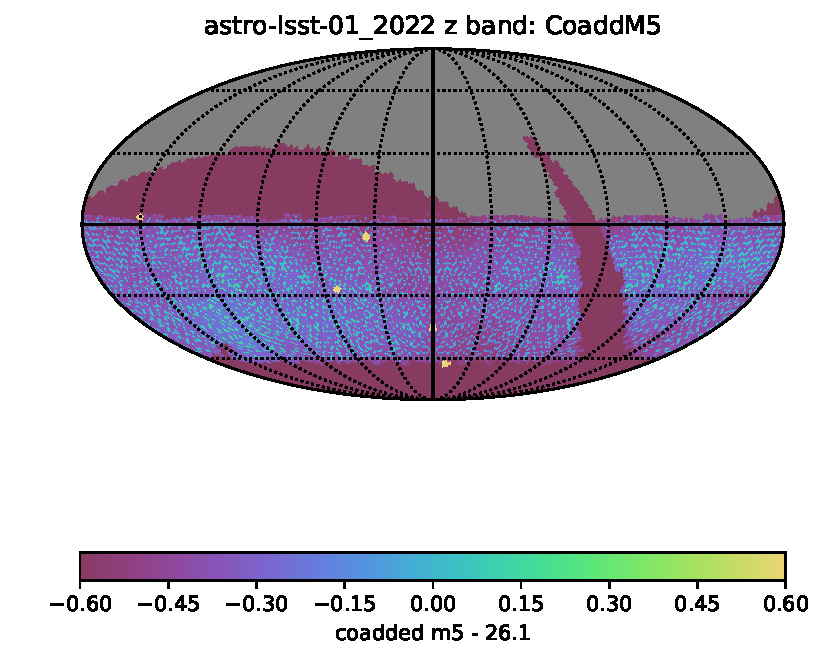
\includegraphics[width=0.4\textwidth]{figures/astro-lsst-01_2022_CoaddM5_z_band_HEAL_SkyMap}
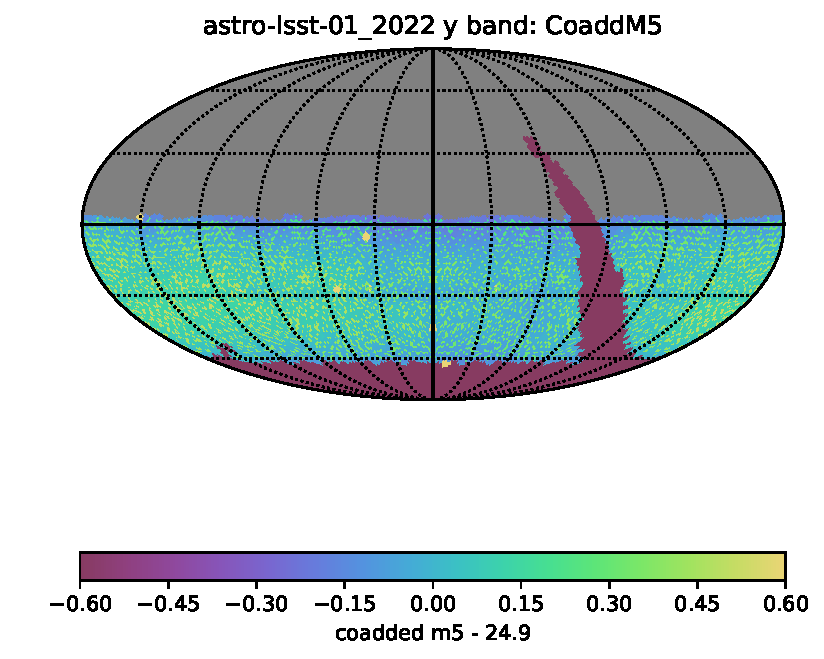
\includegraphics[width=0.4\textwidth]{figures/astro-lsst-01_2022_CoaddM5_y_band_HEAL_SkyMap}
\caption{Coadded depth per filter for astro-lsst-01\_2022.
\label{fig:baseline_coadd}}
\end{figure}


\section{Known issues}

There are some known issues with astro-lsst-01\_2022, common to all \opsim v4 simulated surveys produced with \opsim v4.1.0. to 4.1.0.10.

There are some visits with higher than expected seeingFwhmEff values - even as large as 4.1". This is because the configuration files specify a cutoff for `seeing', but the scheduler only knows about the zenith value of the seeing when deciding whether a visit could be scheduled or not (rather than the seeing at the location of the field). Thus, some visits have a seeingFwhmEff which exceeds the configuration parameters due to the airmass at which the field was observed -- the seeing at zenith at the same time was within the limits.

There are occasional $u$ band visits during twilight. This is because the filter for a particular visit is chosen based on a combination of what observations have already been obtained, what filter is currently in the camera and in use, and hard limits on the sky brightness. With the new \simsky values for sky brightness, the twilight sky background can be within the cutoff limits even for $u$ band -- especially near zenith and on particularly dark nights. Thus, observing in $u$ band during twilight doesn't violate any of the configuration constraints because the sky is dark enough to meet the constraint. It is impossible, with a simple hard constraint, to choose a value that permits observing in $u$ band at a wide range of airmasses and reasonable range of lunar phases, while rejecting $u$ band observations during twilight at zenith on dark nights. A similar condition exists for $g$ band.

The visits for astro-lsst-01\_2022, as with all \opsim v3 and v4 runs, are pinned to a fixed tesselation on the sky, without any translational dithering pattern. Different dithering patterns can be applied as an `after burner' via MAF, to smooth out visit coverage over the sky. Due to how these dither patterns may be applied, if visits are pushed out of the main footprint, the resulting values for the fO metrics may fall below the SRD requirements. Better dither patterns, or even better yet, folding dithers back into the scheduler directly, are required.

The camera rotator angle has maximum values at +/- 90 degrees, and must be set to an angle of 0 for filter changes. The current scheduler does not add any particular choice of orientation to the rotator angle, instead simply letting the rotator follow the sky during observations and then holding its angle unchanged during a slew. In addition, in the current scheduler algorithm, if a target would require moving the rotator beyond these limits, the target is simply skipped. In the future, it may be desirable to add a more sophisticated choice of rotator angles, to smooth the distribution of angles used for observing a given field.

These issues will be addressed with updates in a future version of the scheduler.

\section{Reproducibility of new baseline survey and its evaluation}

The astro-lsst-01\_2022  simulated survey was produced using \opsim v4, 4.1.0.10.  This overarching package designation includes, specifically:
\begin{itemize}
\item Observatory model (ts\_observatory\_model) version 1.0.1
\item Astro sky model (ts\_astrosky\_model) version 1.0.0
\item Dateloc (ts\_dateloc) version 1.0.0
\item Sky brightness model (sims\_skybrightness\_pre) version 2.3.7.sims
\item Sky brightness precalculated file version 4f5efe2
\item SOCS (sims\_ocs) version 1.0.1.10
\item Scheduler (ts\_scheduler) version 1.1
\end{itemize}

The configuration parameters were left as the defaults for this version, with the exception that the airmass bonus was set to 0 for all proposals and the $HA$ bonus was set to 0.3, with $HA_{max}$ = 3 hrs for all proposals except Deep Drilling, where it was $HA$ bonus = 0.3 and $HA_{max}$ = 6 hrs. The details of all configuration parameters can be found in the sqlite output database, in the Config table, as well as in the github repo housing this document (\url{https://github.com/lsst-pst/survey_strategy/tree/master/db/baseline-doc/configs}).

The original output file astro-lsst-01\_2022 produced by v4.1.0.10 had a faulty value for seeingFwhmGeom, as a result of a bug in the \socs software. These values have been corrected in the \opsim v4 output files which have been made publicly available, with a comment placed into the Config table that this correction has been made.

The simulated survey output database, astro-lsst-01\_2022.db, is available in the github repo housing this document, together with MAF analysis outputs. These MAF outputs can also be found online at \url{http://astro-lsst-01.washington.edu:8081}.

\section{Details of astro-lsst-01\_2022}



%%%%%%%%%%%%%%%%%%%%%%%%%%%%%%%%%
\begin{figure}[ht]
\centering
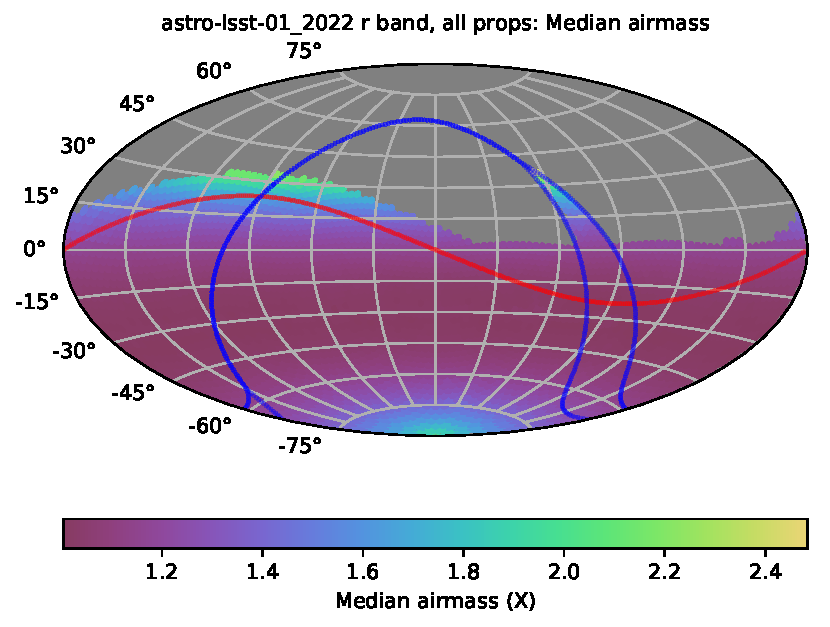
\includegraphics[width=0.49\textwidth]{figures/astro-lsst-01_2022_Median_airmass_r_band_all_props_OPSI_SkyMap}
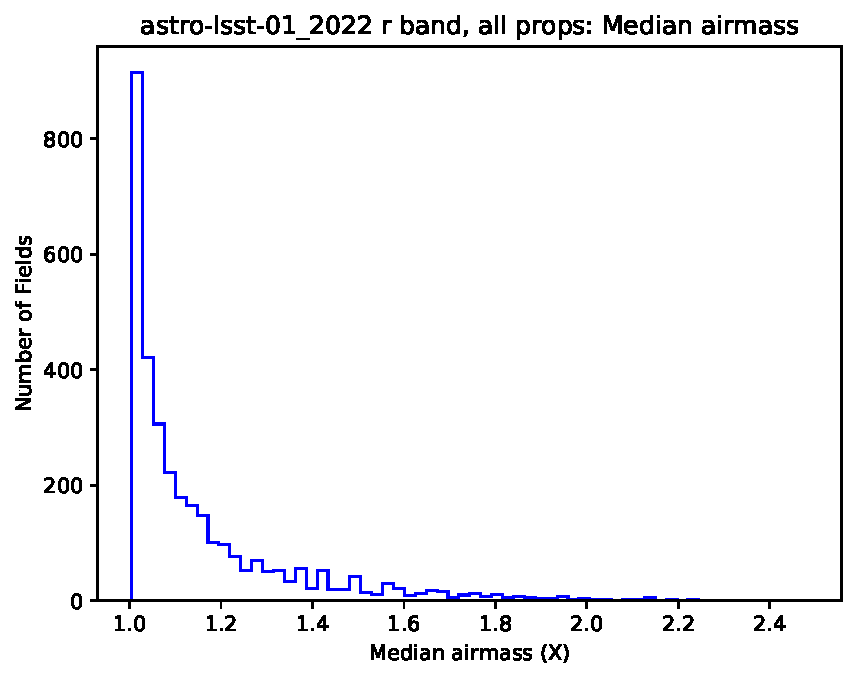
\includegraphics[width=0.49\textwidth]{figures/astro-lsst-01_2022_Median_airmass_r_band_all_props_OPSI_Histogram}
%\vskip -1.3in
\caption{The median airmass in the $r$ band across the sky for simulated cadence
astro-lsst-01\_2022 is shown in Aitoff projection of equatorial coordinates
in the left panel. The red line shows the Ecliptic and the blue line shows the Galactic
equator. The blue curve splits to enclose the so-called ``Galactic confusion zone''. The corresponding
airmass histogram is shown in the right panel. For the main survey area, the maximum
allowed airmass was set to 1.5. }
\label{fig:baseline_airmass}
\end{figure}
%%%%%%%%%%%%%%%%%%%%%%%%%%%%%%%%%

%%%%%%%%%%%%%%%%%%%%%%%%%%%%%%%%%
\begin{figure}[t!]
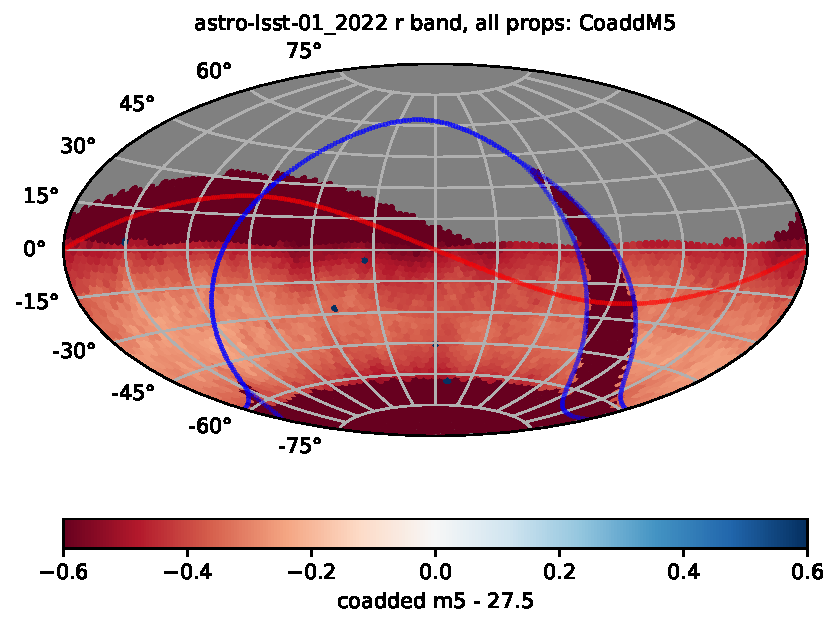
\includegraphics[angle=0,width=0.99\hsize,clip]{figures/astro-lsst-01_2022_CoaddM5_r_band_all_props_OPSI_SkyMap}
\caption{The coadded $5\sigma$ depth for point sources in the $r$ band
across the sky at the end of 10 years for simulated cadence astro-lsst-01\_2022 is shown
in Aitoff projection of equatorial coordinates. The red line shows the Ecliptic and
the blue line shows the Galactic equator (it bifurcates around the so-called
``Galactic confusion zone''). The median value across the WFD Cadence area
is 27.2, with RMS scatter of 0.07 mag. The small dark dots are Deep Drilling
fields, with a median $5\sigma$ depth of 28.7.}
\label{fig:baseline_coaddm5}
\end{figure}
%%%%%%%%%%%%%%%%%%%%%%%%%%%%%%%%%


%%%%%%%%%%%%%%%%%%%%%%%%%%%%%%%%%
\begin{figure}[t!]
\centering
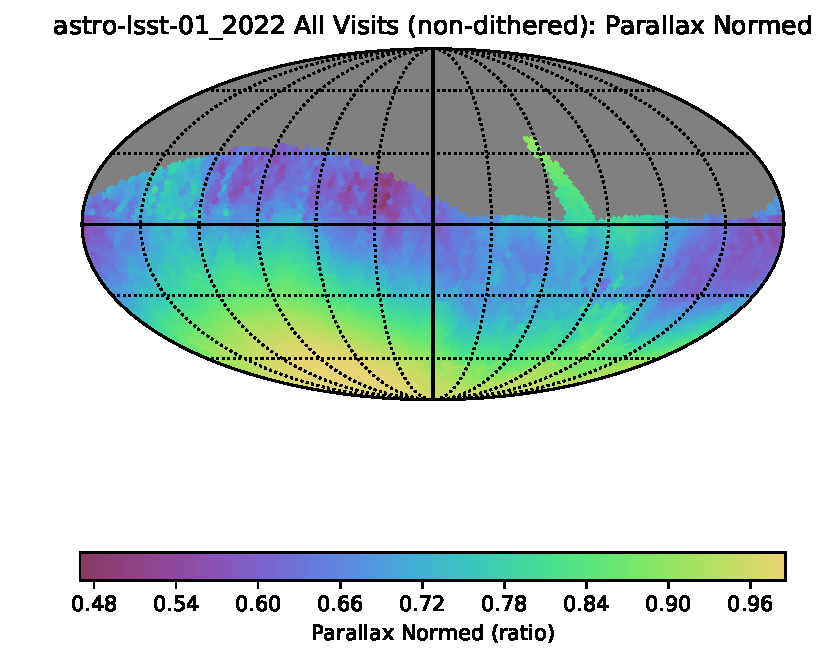
\includegraphics[width=0.4\textwidth]{figures/astro-lsst-01_2022_Parallax_Normed_All_Visits_non-dithered_HEAL_SkyMap.pdf}
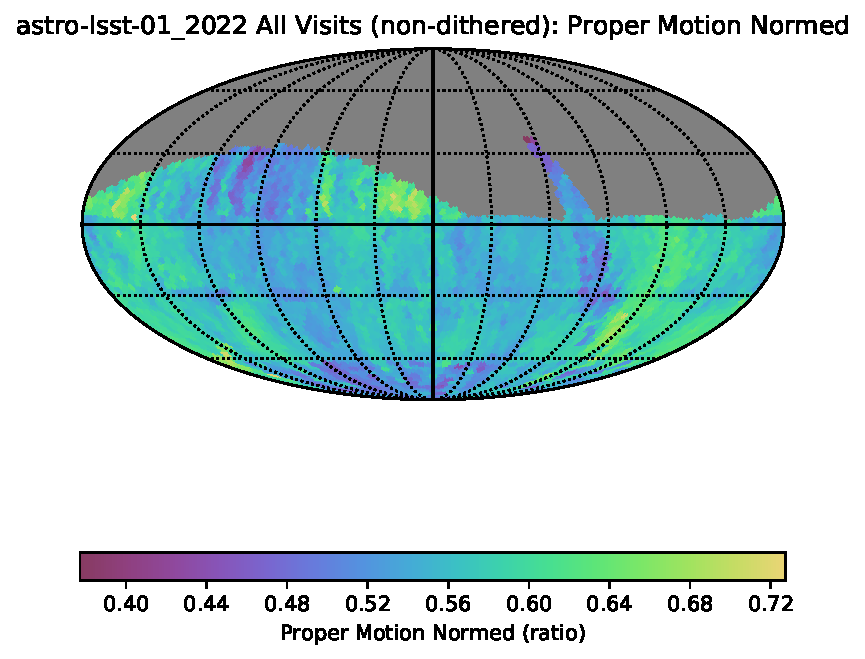
\includegraphics[width=0.4\textwidth]{figures/astro-lsst-01_2022_Proper_Motion_Normed_All_Visits_non-dithered_HEAL_SkyMap.pdf} \\
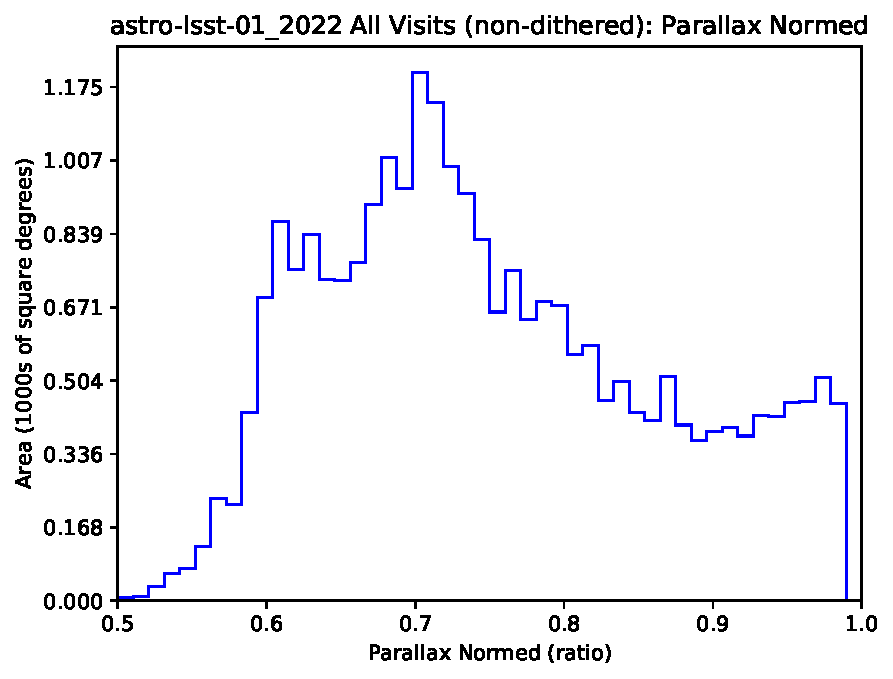
\includegraphics[width=0.4\textwidth]{figures/astro-lsst-01_2022_Parallax_Normed_All_Visits_non-dithered_HEAL_Histogram.pdf}
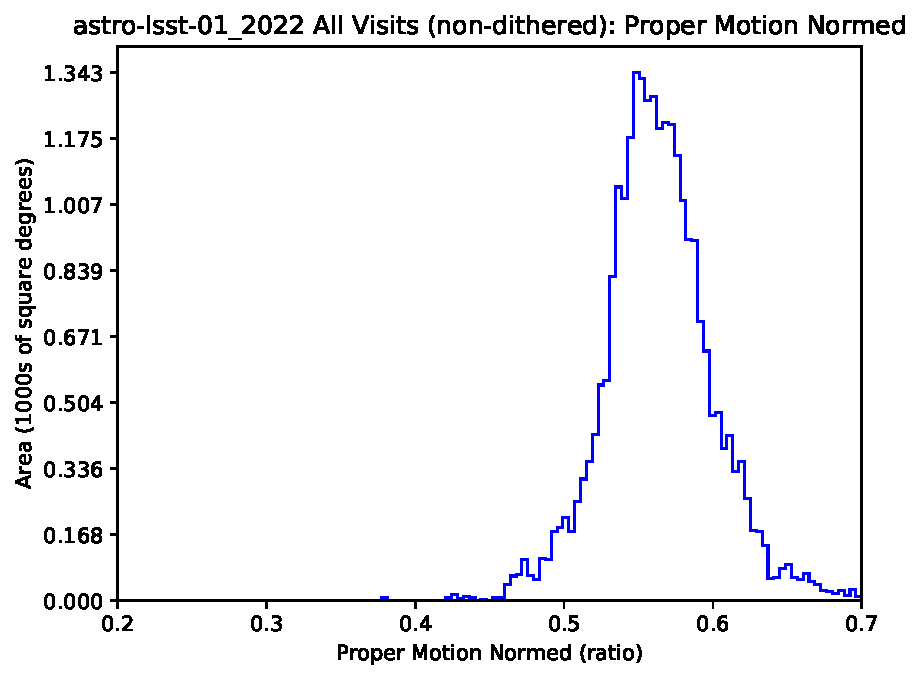
\includegraphics[width=0.4\textwidth]{figures/astro-lsst-01_2022_Proper_Motion_Normed_All_Visits_non-dithered_HEAL_Histogram.pdf}
\caption{The trigonometric parallax errors (left) and proper motion errors (right), normalized
by the values for idealized perfectly optimized cadences (parallax: all the observations are taken
at maximum parallax factor, resulting in a peak at the South Ecliptic pole; proper motion:
a half of all visits are obtained on the first day and the rest on the last day of the survey),
obtained for simulated cadence astro-lsst-01\_2022 are shown in Aitoff projection of equatorial
coordinates.}
\label{fig:baseline_parapm}
\end{figure}
%%%%%%%%%%%%%%%%%%%%%%%%%%%%%%%%%


The Baseline Cadence,
astro-lsst-01\_2022, has the following basic
properties
\begin{enumerate}
\item The total number of visits is 2,372,700, with 86.0\% spent on
the main Wide, Fast, Deep (WFD) survey, 5.0\% on the
North Ecliptic Spur proposal, 1.6\% on the Galactic Plane proposal, 2.0\%
on the South Celestial Pole proposal, and 5.0\% on the Deep Drilling
Cosmology proposal (5 fields).\footnote{The community-contributed white papers leading to the
Deep Drilling fields defined in the Baseline Cadence can be found via
\url{https://community.lsst.org/t/deep-drilling-whitepapers/732}.}
\item The median number of visits per night is 785, the range is
139 to 1082, with 3,025 observing nights. The mean slew time is 7.92
seconds (median: 5.17 sec) and the total exposure time (after 10 yeras) is 71.2 Msec (total number of visits $\times$ mean exposure time).
The surveying efficiency, or the median total open shutter time (per night)
as a fraction of the observing time (the ratio of the open shutter time to
the sum of the open shutter time, readout time and slew time) is 72\%.
\item
The 25\%-75\% quartiles for the number of filter changes per night are 1
and 4, with the mean of 3.13 The total number of filter changes through the survey is 10,644.
\item In the $r$ band, the median effective seeing for all proposals is 0.86 arcsec.
The median airmass for all filters and all proposals is 1.08.
The median single-visit $5\sigma$ depth for point sources in $r$ band in the WFD area is 24.27 (using the best
current estimate of the fiducial depth at airmass of one, $m_5(r)=24.39$,
defined by the SRD Table 5). The variation of the median airmass for the $r$
band observations with the position on the sky is shown in
\autoref{fig:baseline_airmass}.
\item The median single-visit depths for WFD fields are (23.32, 24.63, 24.27,
23.70, 22.79, 22.00) in the $ugrizy$ bands.
% \footnote{Note that these values
% depend on externally supplied values for fiducial zenith dark time single-epoch
% $5\sigma$ depths; the following values were used in analysis described
% here: (23.62, 24.85, 24.39, 23.94, 23.36, 22.45) in the $ugrizy$
% bands, respectively. These values are similar, but not identical, to the values
% listed in Table 2 from the latest version (v3.1) of the LSST overview
% paper: (23.68, 24.89, 24.43, 24.00, 23.45, 22.60). This discrepancy
% is due to continuing improvements in the system performance estimates.}.
% These values are shallower than
% the zenith dark time values for three main reasons: the sky is expected to be
% brighter for non-dark time and away from zenith, the sky brightness model
% currently implemented in \OpSim has some shortcomings (a new model has been implemented for version 4),
% and the moon avoidance is not as aggressive
% as it could be (many observations are taken very close to the moon avoidance limit of 30 degrees,
% rather than farther away where the sky is darker). As a result, the median limiting depths
% above are brighter than typical zenith dark-time images by close
% to 1 mag in the $z$ and $y$ bands, and a few tenths of a magnitude in the
% $u$, $g$ and $i$ bands.
\item For the 2,293 (overlapping) fields from the WFD area,
the median number of visits in the $ugrizy$ bands is (61, 85, 194, 193, 180,
179), respectively. These medians exceed the requested
number of visits (design specification from the SRD\footnote{The LSST
Science Requirements Document (SRD) is available as
\url{http://ls.st/lpm-17}}) of (56, 80, 184, 184, 160, 160) in the $ugrizy$
bands.
\item The median coadded $5\sigma$ depth
for point sources in the $ugrizy$ bands is (25.6, 27.1, 27.2, 26.6,
25.7, 24.9), respectively, for the WFD area. The distribution
of coadded depth across the sky is fairly uniform, as illustrated in \autoref{fig:baseline_coaddm5}.
% Do we still need this FWHMgeom
% \item For the 2,293 fields from the WFD area, the median
% geometric FWHM for seeing is 0.78 arcsec in the $r$ band and 0.77 arcsec
% in the $i$ band. The median airmass in the $urz$ bands is 1.25, 1.20 and 1.26
% (the maximum allowed airmass for the WFD area was set to
% 1.5).  The median sky brightness in the $ury$ bands is 22.0 mag/arcsec$^2$,
% 21.1 mag/arcsec$^2$, and 17.3 mag/arcsec$^2$, respectively (for comparison, the
% assumed dark sky brightness at zenith in the $ury$ bands is 23.0, 21.2 and 18.6
% mag/arcsec$^2$).  The current model sky brightness in the $y$ band is biased
% very high because most $y$ band (and many $z$ band) observations are taken in twilight where \OpSim currently uses a very simple (and bright) sky model.
\item Restricted to the WFD fields, a unique area of
18,000 square degrees received at least 835 visits per field (summed over bands;
the SRD design value is 825).
\item The median trigonometric parallax and proper motion errors are
0.57 mas and 0.14 mas/yr, respectively, for bright sources (limited by
assumed systematic errors in relative astrometry of 10 mas), and 5.1
mas and 1.3 mas/yr for points sources with $r=24$ (assuming flat
spectral energy distribution), over the WFD fields. The variation of parallax
and proper motion errors across the sky is visualized in \autoref{fig:baseline_parapm}.
\end{enumerate}


%%%%%%%%%%%%%%%%%%%%%%%%%%%%%%%%%
\begin{figure}[t!]
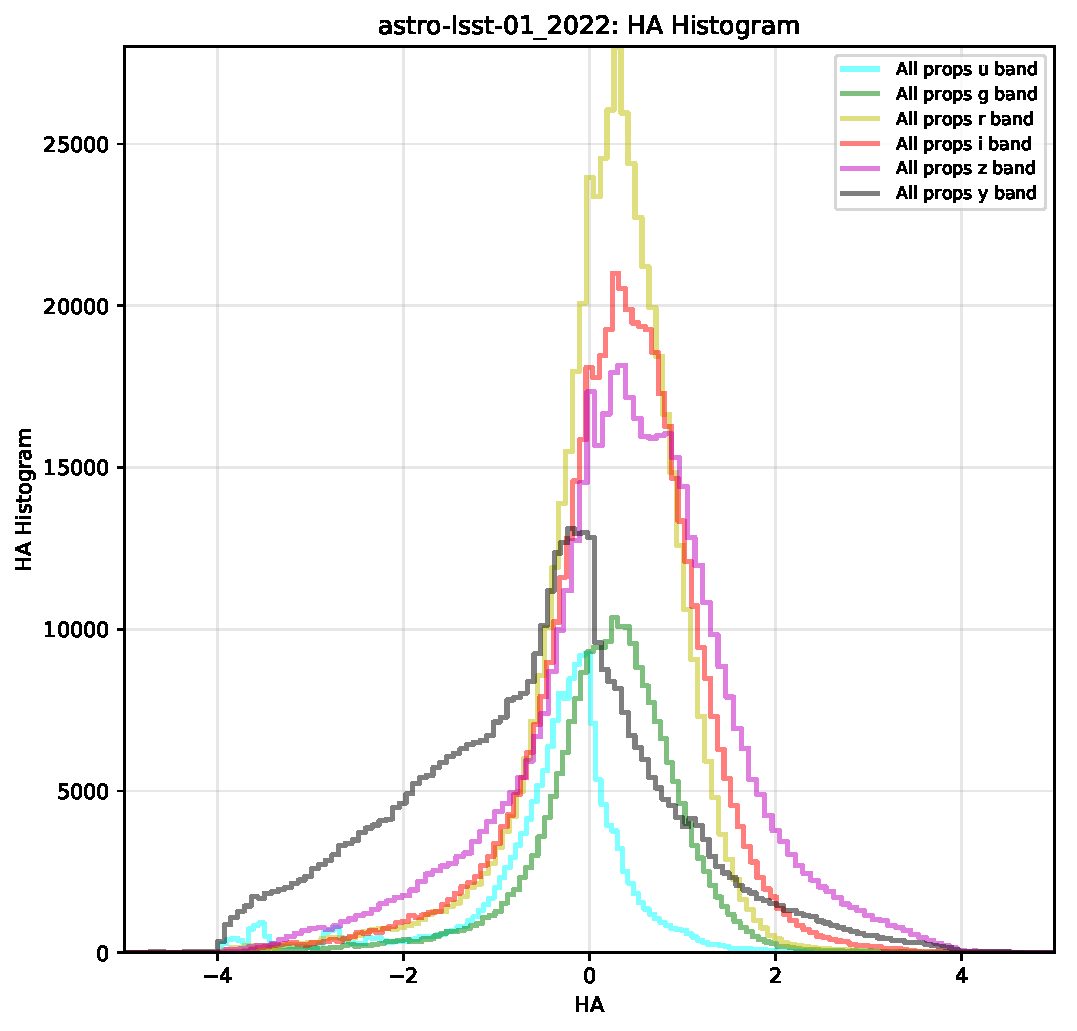
\includegraphics[width=0.49\textwidth]{figures/astro-lsst-01_2022-ha_hist_per_filter.pdf}
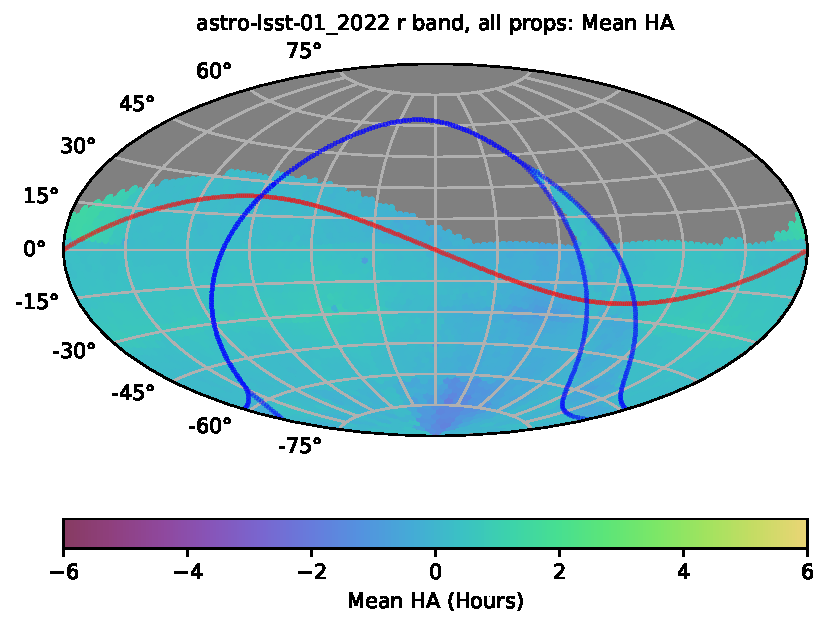
\includegraphics[width=0.49\textwidth]{figures/astro-lsst-01_2022_Mean_HA_r_band_all_props_OPSI_SkyMap.pdf}
\caption{Histograms in the left panel show the distribution of hour angles (HA) in
6 bands for all proposals from simulated cadence astro-lsst-01\_2022.
The right panel shows the distribution across the sky of the mean HA for
all observations in the $r$ band. }
\label{fig:baseline_ha}
\end{figure}
%%%%%%%%%%%%%%%%%%%%%%%%%%%%%%%%%

%%%%%%%%%%%%%%%%%%%%%%%%%%%%%%%%%
\begin{figure}[t!]
\vskip -0.0in
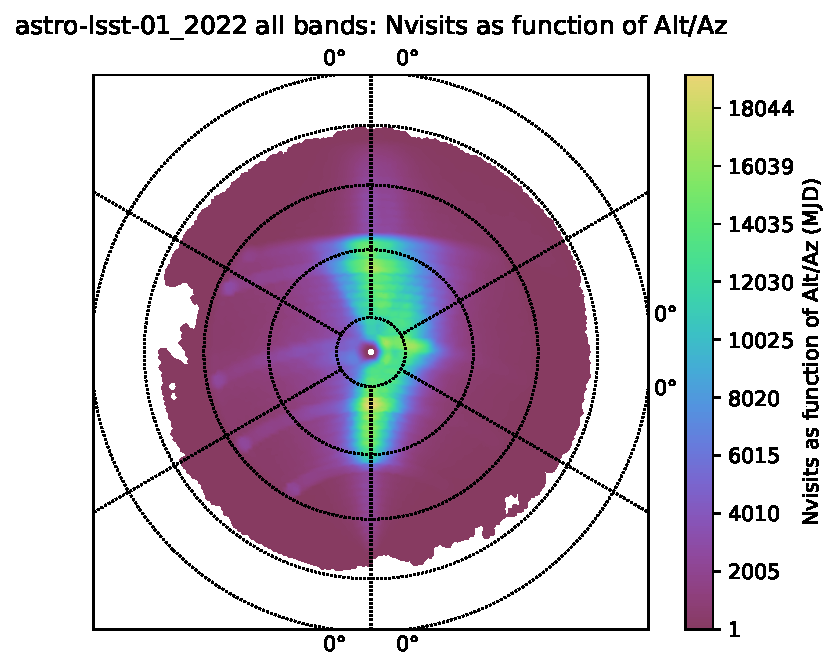
\includegraphics[angle=0,width=0.49\hsize,clip]{figures/astro-lsst-01_2022_Nvisits_as_function_of_Alt_Az_all_observations_HEAL_SkyMap.pdf}
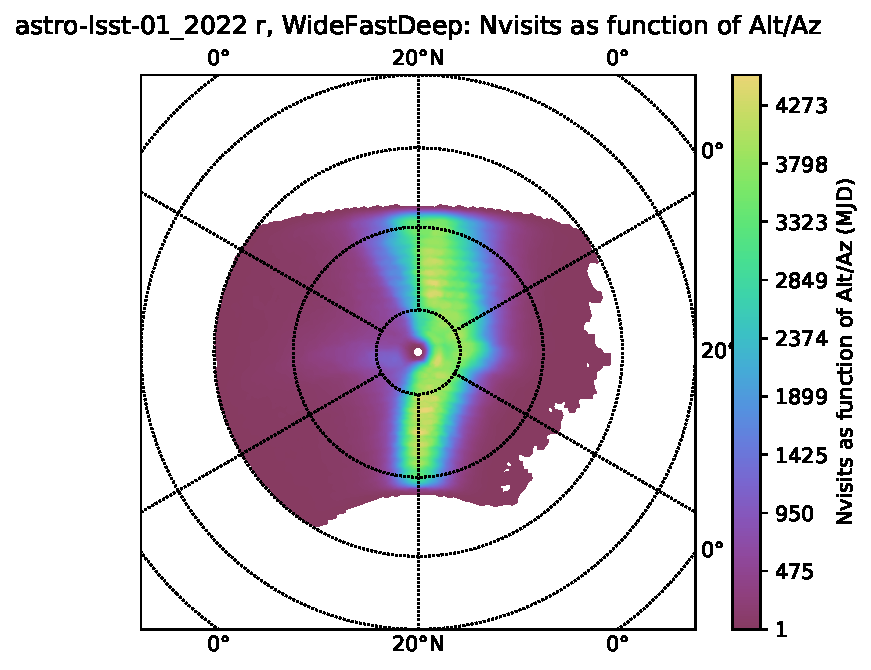
\includegraphics[angle=0,width=0.49\hsize,clip]{figures/astro-lsst-01_2022_Nvisits_as_function_of_Alt_Az_r_WideFastDeep_HEAL_SkyMap.pdf}
\vskip -0.1in
\caption{The color-coded map in the left panel shows the visit count from the
Baseline Cadence simulation astro-lsst-01\_2022 in the equal-area Lambert projection of the
horizontal coordinate system (altitude-azimuth), with north on top and west towards the
right, for all six bands and proposals (Wide, Fast, Deep, Galactic Plane, Deep Drilling
fields, North Ecliptic Spur, and South Celestial Pole region). The right panel is analogous,
but only shows the $r$ band visits for WFD fields.}
\label{fig:baseline_AltAz}
\end{figure}
%%%%%%%%%%%%%%%%%%%%%%%%%%%%%%%%%

%%%%%%%%%%%%%%%%%%%%%%%%%%%%%%%%%
\begin{figure}[th!]
\vskip -0.0in
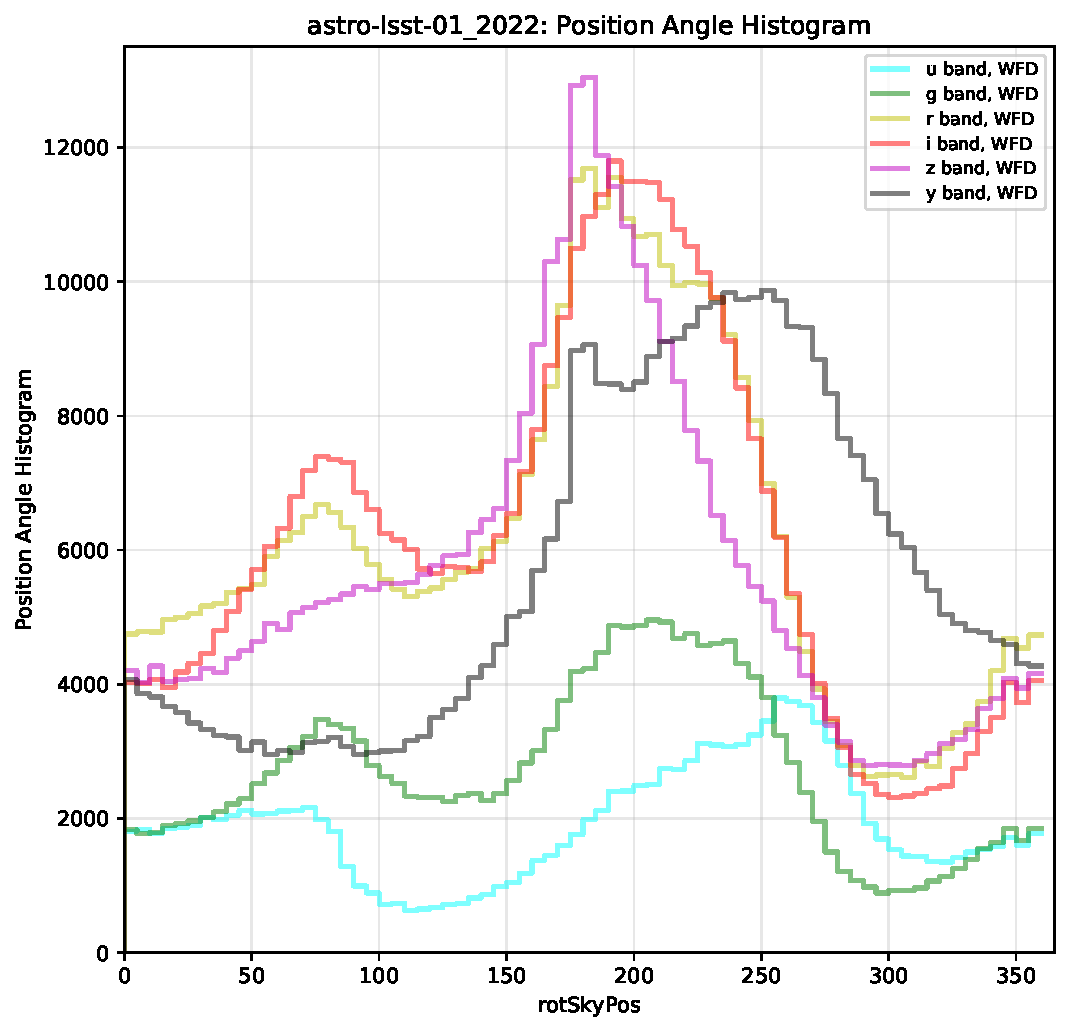
\includegraphics[angle=0,width=0.49\hsize,clip]{figures/astro-lsst-01_2022-rotpos_hist_per_filter.pdf}
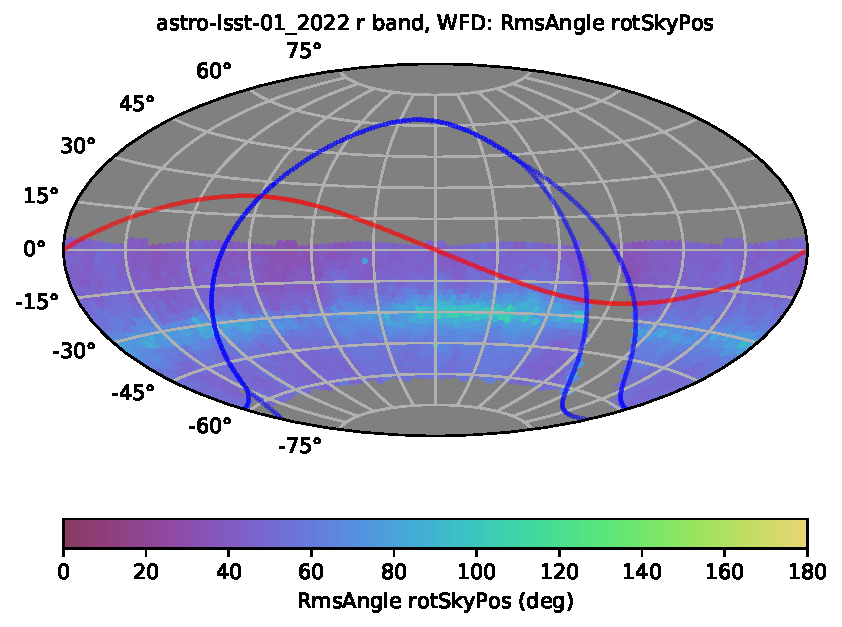
\includegraphics[angle=0,width=0.49\hsize,clip]{figures/astro-lsst-01_2022_RmsAngle_rotSkyPos_r_band_WFD_OPSI_SkyMap.pdf}
\vskip -0.1in
\caption{The left panel shows the position angle distribution (in degrees) in each band for the
main survey fields in astro-lsst-01\_2022. The position angle is the angle between
``up'' in the image and North on the sky. The variation of the root-mean-square scatter of the
$r$ band distribution across the sky is shown in the right panel.}
\label{fig:baseline_rotator}
\end{figure}
%%%%%%%%%%%%%%%%%%%%%%%%%%%%%%%%%

%%%%%%%%%%%%%%%%%%%%%%%%%%%%%%%%%
\begin{figure}[t!]
\vskip -0.0in
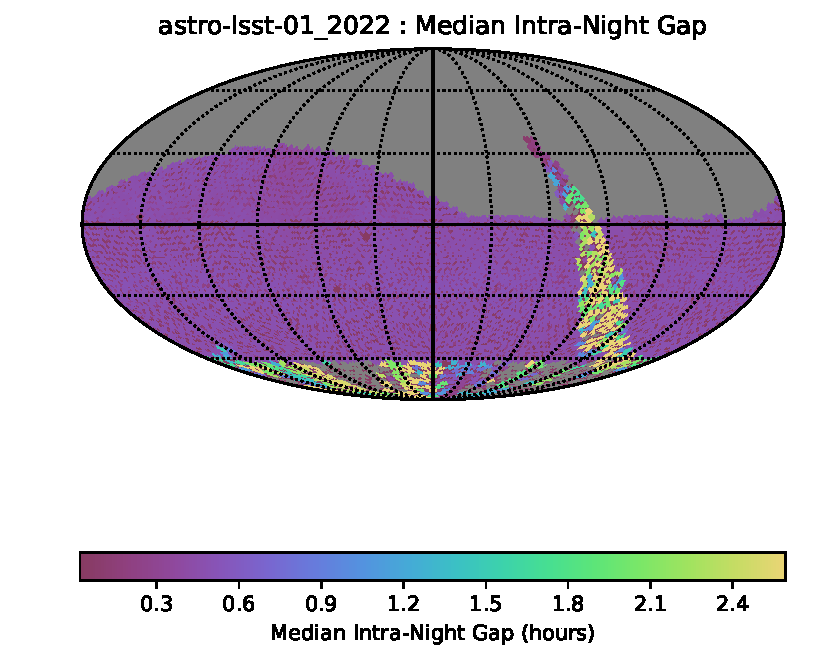
\includegraphics[angle=0,width=0.49\hsize,clip]{figures/astro-lsst-01_2022_Median_Intra-Night_Gap_HEAL_SkyMap.pdf}
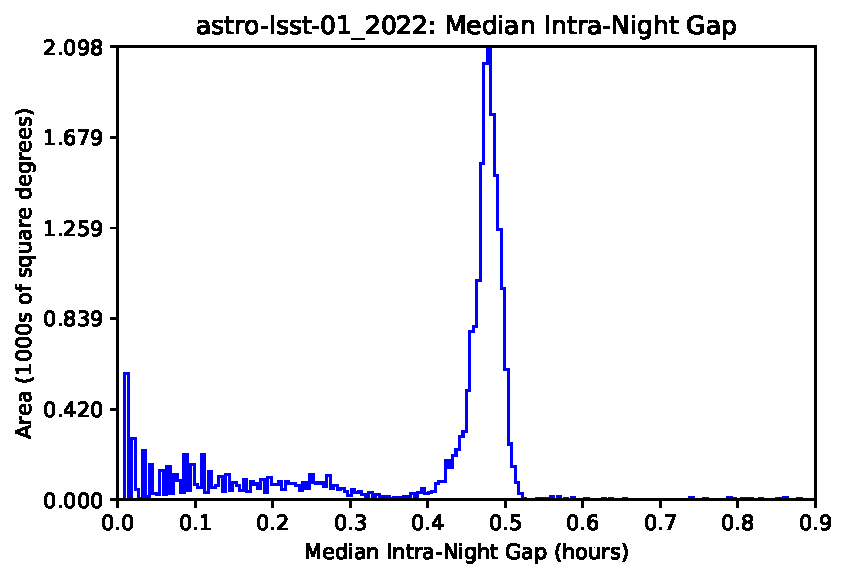
\includegraphics[angle=0,width=0.49\hsize,clip]{figures/astro-lsst-01_2022-median_intra_night_gap_hist.pdf}
\vskip -0.1in
\caption{The median intra-night gap (or revisit time) is shown in Aitoff projection
for all proposals and all filters for the Baseline Cadence astro-lsst-01\_2022.
On average, when a field is observed multiple times in a night there is a 28 minute gap between the observations.}
\label{fig:baseline_InterGapAll}
\end{figure}
%%%%%%%%%%%%%%%%%%%%%%%%%%%%%%%%%

%%%%%%%%%%%%%%%%%%%%%%%%%%%%%%%%%
\begin{figure}[t!]
\vskip -0.0in
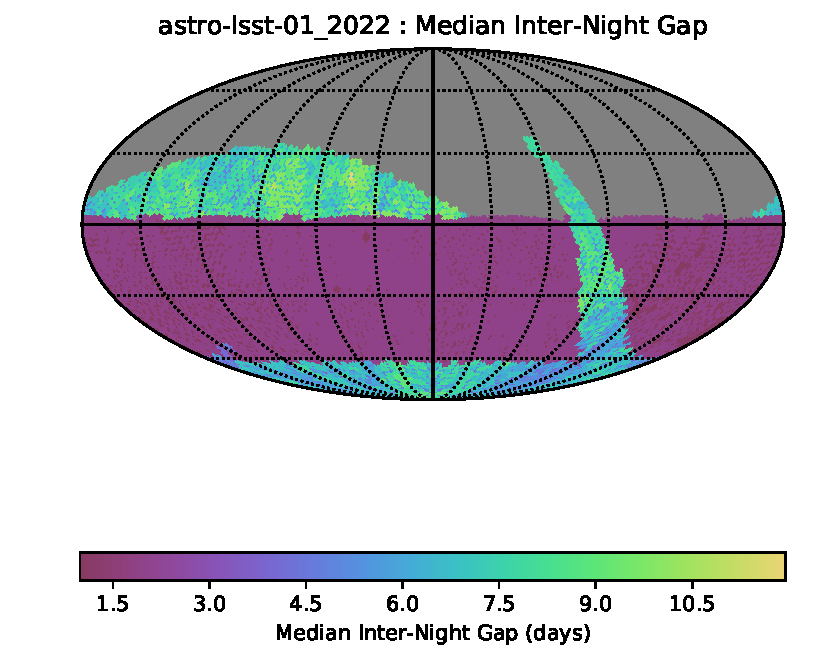
\includegraphics[angle=0,width=0.49\hsize,clip]{figures/astro-lsst-01_2022_Median_Inter-Night_Gap_HEAL_SkyMap.pdf}
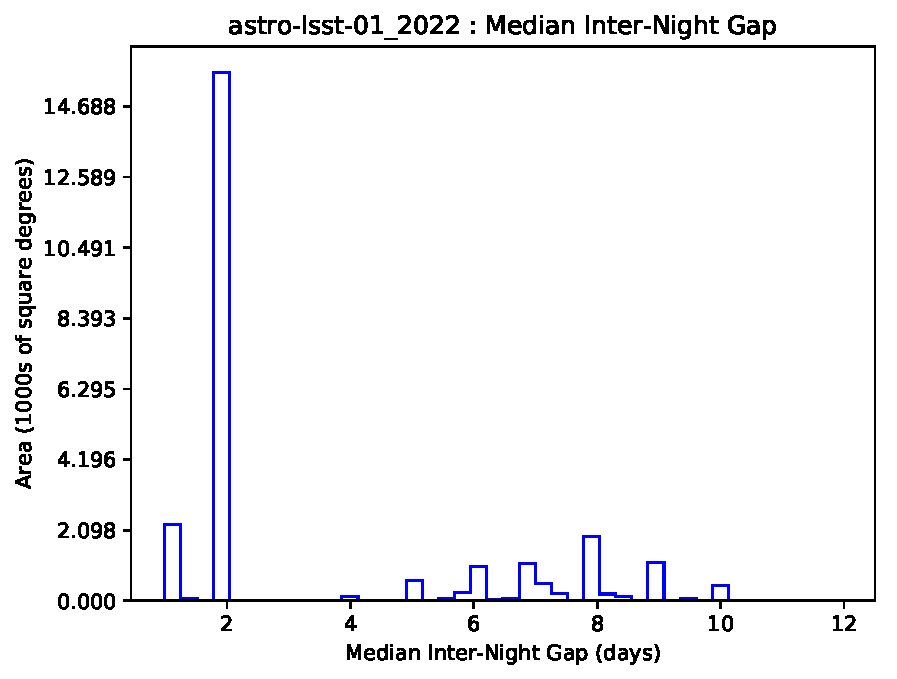
\includegraphics[angle=0,width=0.49\hsize,clip]{figures/astro-lsst-01_2022_Median_Inter-Night_Gap_HEAL_Histogram.pdf}
\vskip -0.1in
\caption{The median inter-night gap (or revisit time) is shown in Aitoff projection
for all proposals and all filters for the Baseline Cadence astro-lsst-01\_2022.
On average, fields in the main survey get revisited about every 2 days.}
\label{fig:baseline_GapAll}
\end{figure}
%%%%%%%%%%%%%%%%%%%%%%%%%%%%%%%%%


%%%%%%%%%%%%%%%%%%%%%%%%%%%%%%%%%
\begin{figure}[h!]
\vskip -0.0in
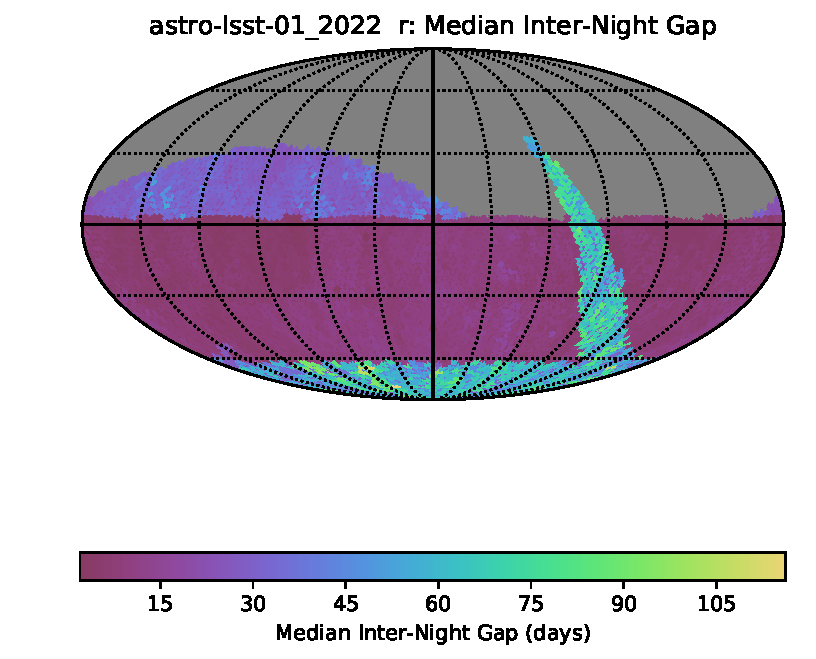
\includegraphics[angle=0,width=0.49\hsize,clip]{figures/astro-lsst-01_2022_Median_Inter-Night_Gap_r_HEAL_SkyMap.pdf}
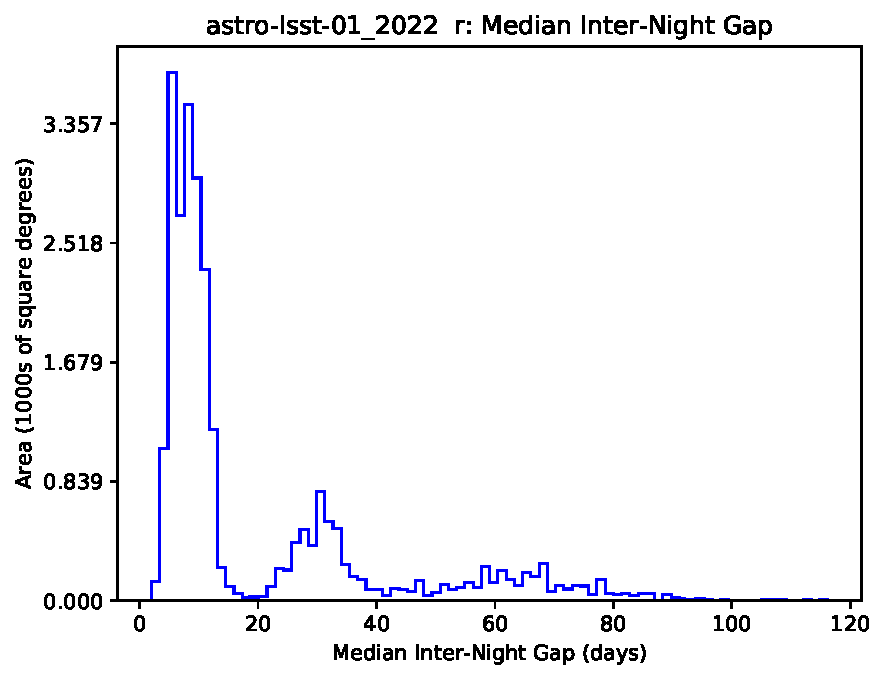
\includegraphics[angle=0,width=0.49\hsize,clip]{figures/astro-lsst-01_2022_Median_Inter-Night_Gap_r_HEAL_Histogram.pdf}
\vskip -0.1in
\caption{The median inter-night gap for $r$ band visits is shown in Aitoff projection
for all proposals for the Baseline Cadence astro-lsst-01\_2022.
On average, fields in the main survey get revisited in the $r$ band about every two weeks.}
\label{fig:baseline_Gapr}
\end{figure}
%%%%%%%%%%%%%%%%%%%%%%%%%%%%%%%%%

%%%%%%%%%%%%%%%%%%%%%%%%%%%%%%%%%
\begin{figure}[t!]
\vskip -0.0in
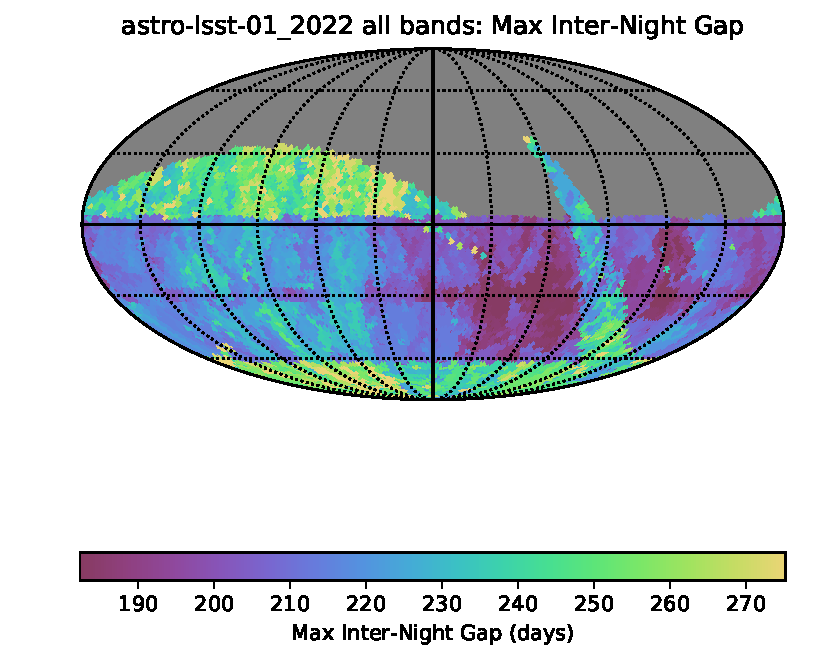
\includegraphics[angle=0,width=0.49\hsize,clip]{figures/astro-lsst-01_2022_Max_Inter-Night_Gap_all_bands_HEAL_SkyMap.pdf}
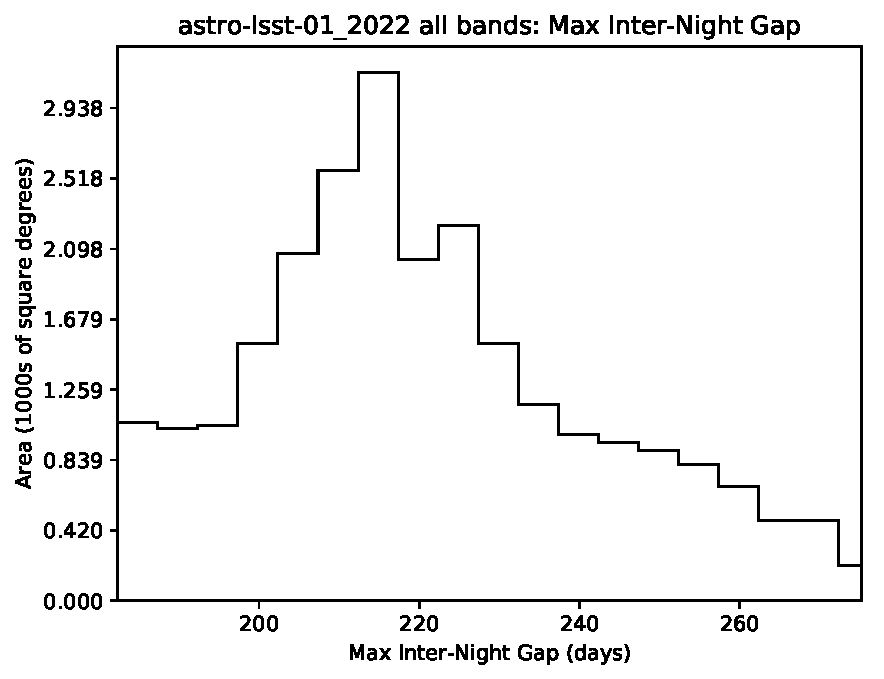
\includegraphics[angle=0,width=0.49\hsize,clip]{figures/astro-lsst-01_2022_Max_Inter-Night_Gap_all_bands_HEAL_Histogram.pdf}
\vskip -0.1in
\caption{The maximum inter-night gap (or revisit time) is shown in Aitoff projection
for all proposals and all filters for the Baseline Cadence astro-lsst-01\_2022.}
\label{fig:baseline_MAXGapAll}
\end{figure}
%%%%%%%%%%%%%%%%%%%%%%%%%%%%%%%%%

%%%%%%%%%%%%%%%%%%%%%%%%%%%%%%%%%
\begin{figure}[h!]
\vskip -0.0in
\includegraphics[angle=0,width=0.49\hsize,clip]{figures/astro-lsst-01_2022_SNAlert_non-dithered_HEAL_SkyMap.pdf}
\includegraphics[angle=0,width=0.49\hsize,clip]{figures/astro-lsst-01_2022_SNAlert_non-dithered_HEAL_Histogram.pdf}
\vskip -0.1in

\caption{The fraction of simulated Type Ia SNe at a redshift of 0.5 detected
pre-peak in any filter for the Baseline Cadence astro-lsst-01\_2022. About
40\% of all such SNe from the main survey will be detected before their
maximum brightness.}
\label{fig:baseline_EarlySNe}
\end{figure}
%%%%%%%%%%%%%%%%%%%%%%%%%%%%%%%%%

Here we only provide the basic
performance parameters of the special proposals. The
North Ecliptic Spur proposal (5.0\% of the observing time) obtained  245 visits per field, summed over $griz$ bands. These
fields are placed along the northern part of the Ecliptic. The
Galactic Plane proposal (1.6\%) obtained (27, 27, 27, 27, 29, 30) visits in $ugrizy$, respectively, per field
across the region extending in Galactic latitude 10 degrees
from the Galactic center, with the boundary approaching the Galactic
equator linearly with longitude, and the zone ending at $l=90$ deg.
and at $l=270$ deg. The South Celestial Pole proposal (2.0\%) obtained
obtained (26, 26, 26, 26, 28, 38) visits in $ugrizy$, respectively, for fields centers with Dec $<
-62.5$ deg. The Deep Drilling proposal (5.0\%) included 5
fields, with each obtaining several thousand visits per band as required for various cosmology investigations. The
coadded $5\sigma$ depths for these fields are much fainter than for
the main survey: the median values are (27.9, 28.6, 28.7, 28.2, 27.8,
26.1) in the $ugrizy$ bands, respectively.

% Include all the relevant bib files.
% https://lsst-texmf.lsst.io/lsstdoc.html#bibliographies
\bibliography{lsst,lsst-dm,refs_ads,refs,books}

\end{document}
